% Monarch of the Hill group report (AME 101, Fall 2026, Team 2)
% Compile with pdfLaTeX (Overleaf default). Body text lives in sections/.

\documentclass[12pt,letterpaper]{article}

% ---------------------------------------------------------------------------
% Draft switch: \showtbdtrue highlights every open placeholder in yellow.
% Set to \showtbdfalse for the final PDF only once no \tbd{} remain;
% with it off, any leftover \tbd{} prints as plain bracketed text.
% ---------------------------------------------------------------------------
\newif\ifshowtbd
\showtbdtrue

% Fonts and page
\usepackage[T1]{fontenc}
\usepackage[utf8]{inputenc}
\usepackage{newtxtext}
\usepackage{newtxmath}
\usepackage[scaled=0.92]{inconsolata}
\usepackage[letterpaper,margin=1in]{geometry}
\usepackage[final]{microtype}
\usepackage{setspace}
\setstretch{1.05}
\setlength{\parindent}{0pt}
\setlength{\parskip}{0.55\baselineskip}
\raggedbottom

% Math, units, symbols
\usepackage{amsmath}
\usepackage{bm}
\usepackage[per-mode=symbol,detect-all]{siunitx}
\sisetup{inter-unit-product=\ensuremath{\cdot},range-phrase=\text{ to },range-units=single,list-units=single,product-units=single}
\DeclareSIUnit\inch{in}
\DeclareSIUnit\lbf{lbf}
\DeclareSIUnit\rpm{rpm}

% Figures and tables
\usepackage{graphicx}
\graphicspath{{figures/}}
\usepackage{booktabs}
\usepackage{tabularx}
\usepackage{array}
\newcolumntype{L}{>{\raggedright\arraybackslash}X}
\newcolumntype{C}{>{\centering\arraybackslash}X}
\usepackage[font=small,labelfont=bf,labelsep=period,justification=justified,singlelinecheck=true,skip=6pt]{caption}
\captionsetup[table]{position=top}
\usepackage[section]{placeins}
\setlength{\textfloatsep}{14pt plus 4pt minus 4pt}
\setlength{\floatsep}{12pt plus 3pt minus 3pt}
\renewcommand{\arraystretch}{1.15}

% Lists
\usepackage{enumitem}
\setlist[itemize]{topsep=0pt,partopsep=0pt,itemsep=0.3\baselineskip,parsep=0pt,leftmargin=1.6em}

% Placeholders and highlights
\usepackage{xcolor}
\definecolor{tbdyellow}{HTML}{FFF29A}
\definecolor{linkblue}{HTML}{1F4E8C}
\usepackage{soul}
\sethlcolor{tbdyellow}
\usepackage{tikz}
\ifshowtbd
  \newcommand{\tbd}[1]{\hl{[#1]}}
\else
  \newcommand{\tbd}[1]{[#1]}
\fi
% \placeholderfig{height}{text}: a dashed yellow box where a figure still has to go
\newcommand{\placeholderfig}[2]{%
  \begin{tikzpicture}
    \node[draw=black!65,dashed,line width=0.8pt,fill=tbdyellow,
          minimum width=0.92\linewidth,minimum height=#1,
          text width=0.8\linewidth,align=center,font=\small]{#2};
  \end{tikzpicture}}

% Headings: numbered, bold, no color
\usepackage[explicit]{titlesec}
\titleformat{\section}{\normalfont\large\bfseries}{\thesection}{0.8em}{#1}
\titleformat{\subsection}{\normalfont\normalsize\bfseries}{\thesubsection}{0.8em}{#1}
\titleformat{\paragraph}[runin]{\normalfont\normalsize\bfseries}{}{0pt}{#1.}
\titleformat{name=\section,numberless}{\normalfont\large\bfseries}{}{0pt}{#1}
\titlespacing*{\section}{0pt}{1.6ex plus 0.6ex minus 0.2ex}{0.4ex}
\titlespacing*{\subsection}{0pt}{1.2ex plus 0.4ex minus 0.2ex}{0.2ex}
\titlespacing*{\paragraph}{0pt}{0pt}{0.5em}

% Code listings (Appendix A)
\usepackage{listings}
\lstset{
  language=C++,
  basicstyle=\ttfamily\scriptsize,
  keywordstyle=\bfseries,
  commentstyle=\color{black!60},
  stringstyle=\color{black!80},
  numbers=left,numberstyle=\tiny\color{black!45},numbersep=6pt,
  breaklines=true,breakatwhitespace=false,postbreak=\mbox{$\hookrightarrow$\space},
  columns=fullflexible,keepspaces=true,showstringspaces=false,
  tabsize=4,frame=none,xleftmargin=14pt,
}

% Citations and links (ASME numbered style)
\usepackage[nocompress]{cite}
\renewcommand{\citepunct}{, }
\usepackage[hyphens]{url}
\usepackage[colorlinks=true,linkcolor=black,citecolor=black,urlcolor=linkblue,
            pdftitle={Win the Ground Game, Win the Hill},
            pdfauthor={Gabriel Oliveri, Charlie Haldeman, Efe Altinkaya, Ashley Valdez}]{hyperref}
\urlstyle{same}
\soulregister{\cite}{7}
\soulregister{\ref}{7}
\soulregister{\eqref}{7}

% Table of contents spacing
\usepackage{tocloft}
\setlength{\cftbeforesecskip}{3pt}
\renewcommand{\cftsecfont}{\normalfont}
\renewcommand{\cftsecpagefont}{\normalfont}
\renewcommand{\cfttoctitlefont}{\large\bfseries}
\setlength{\cftbeforetoctitleskip}{0.6ex}
\setlength{\cftaftertoctitleskip}{0.8ex}

% Headers/footers: page number only
\pagestyle{plain}

\begin{document}

% Title page, abstract, contents, nomenclature

\begin{titlepage}
  \centering
  \vspace*{0.4in}
  {\LARGE\bfseries Design and Testing of an Autonomous Tracked Robot for Monarch of the Hill \par}
  \vspace{0.25in}
  {\large Monarch of the Hill, AME 101, Fall 2026\par}
  \vspace{0.3in}
  {\normalsize Team 2: Gabriel Oliveri, Charlie Haldeman, Efe Altinkaya, Ashley Valdez\par}
  \vspace{0.08in}
  {\normalsize University of Southern California\par}
  \vspace{0.4in}
  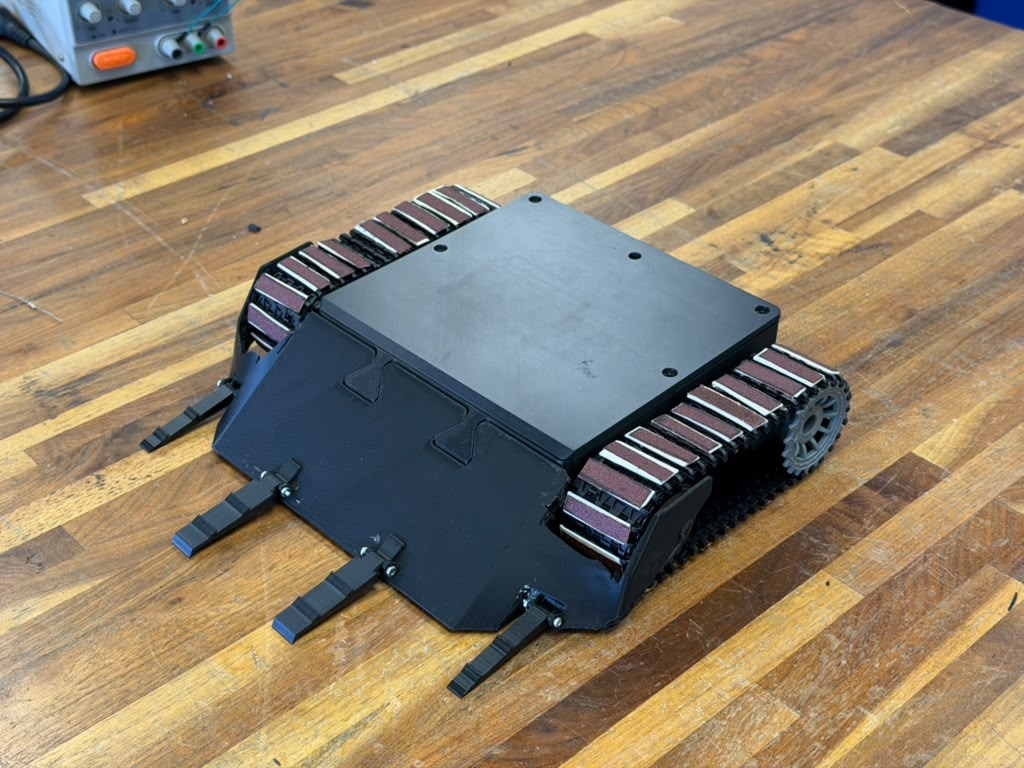
\includegraphics[width=0.62\textwidth]{title_robot.jpg}\par
  \vfill
  \begin{tabular}{@{}lr@{}}
    \toprule
    \textbf{Category} & \textbf{Score} \\
    \midrule
    Organization    & /20 \\
    Documentation   & /35 \\
    Testing         & /25 \\
    Lessons learned & /20 \\
    \midrule
    Total           & /100 \\
    \bottomrule
  \end{tabular}\par
  \vspace*{0.1in}
\end{titlepage}

\setcounter{page}{2}

\section*{Abstract}
\addcontentsline{toc}{section}{Abstract}
We designed and built an autonomous tracked robot for the AME 101 Monarch of the Hill contest. Two robots start at the bottoms of opposite \ang{33.4} ramps, and after \qty{30}{s} the robot whose farthest point is closest to the center of the shared summit wins. Our strategy was to reach the summit first and never depend on a pushing match: a low wedge with forks at the front lets an arriving opponent drive up and over us, and running along a side wall replaces steering. The robot uses two \qty{25}{mm}, \qty{280}{\rpm} gearmotors on the stock sprockets with sandpaper on the tracks, a SparkFun TB6612FNG motor driver and a Particle Photon~2 controller. It tracks its pitch with a complementary filter that combines gyro and accelerometer readings, because the accelerometer alone misreads pitch whenever the robot speeds up or slows down. It climbs the \qty{1.52}{m} ramp in about \qty{3.3}{s} (timed by stopwatch) and weighs \qty{1.000}{kg} against the \qty{1}{kg} limit. We won the contest with a 5--1 record. Our one loss, in the final round, came from run-to-run variation in the timed climb: the robot stopped short on the mesa, and the opponent's farthest point ended up closer to the center. Our main lesson is to triage hard: dropping complex ideas early left enough time to test the robot and its software.

\vspace{0.5\baselineskip}
{\setlength{\parskip}{0pt}\setcounter{tocdepth}{1}\tableofcontents}

\clearpage
\section*{Nomenclature}
\addcontentsline{toc}{section}{Nomenclature}

{\small\renewcommand{\arraystretch}{0.84}
\begin{tabularx}{\textwidth}{@{}l L l@{}}
  \toprule
  \textbf{Symbol} & \textbf{Meaning} & \textbf{Units} \\
  \midrule
  $a$ & acceleration along the ramp & \unit{m/s^2} \\
  $\bm{a}_\mathrm{m}$ & acceleration vector measured by the accelerometer & \unit{m/s^2} \\
  $c$ & distance from the neutral axis to the outermost fiber & \unit{mm} \\
  $F$ & traction force from both tracks & \unit{N} \\
  $F(v)$, $F_\mathrm{stall}$ & drive force from both motors at speed $v$; at stall & \unit{N} \\
  $F_f$ & static friction force between the tracks and the ramp & \unit{N} \\
  $F_\mathrm{att}$, $F_\mathrm{def}$ & largest force an attacker on the ramp can push with; largest force a defender on the mesa can resist with & \unit{N} \\
  $G$ & gear ratio & -- \\
  $g$ & gravitational acceleration, 9.81 & \unit{m/s^2} \\
  $I$ & second moment of area of a section; current drawn from the pack (Eq.~\eqref{eq:vterm}) & \unit{mm^4}; \unit{A} \\
  $I_\mathrm{m}$, $I_\mathrm{stall}$, $I_\mathrm{stall,max}$ & motor current; at stall; largest stall current the pack allows & \unit{A} \\
  $k_\mathrm{t}$ & motor torque constant & \unit{N.m/A} \\
  $k_r$ & resistance factor: total resistance to climbing as a multiple of $m g \sin\ang{33.4}$ & -- \\
  $M$ & bending moment & \unit{N.m} \\
  $m$ & robot mass & \unit{kg} \\
  $N$ & normal force & \unit{N} \\
  $P_\mathrm{max}$ & peak mechanical power per motor & \unit{W} \\
  $R_\mathrm{w}$ & motor winding resistance & \unit{\ohm} \\
  $R_\mathrm{int}$ & pack internal resistance & \unit{\ohm} \\
  $r$ & sprocket rolling radius & \unit{m} \\
  $T$, $T_\mathrm{max}$ & total tension of the tread on the sprocket; tension at which the coupler fails & \unit{N} \\
  $T(G)$ & climb time with gear ratio $G$ & \unit{s} \\
  $T_c$ & filter time constant & \unit{s} \\
  $t_0$ & time constant of the approach to $v_t$ & \unit{s} \\
  $\Delta t$ & filter update interval & \unit{s} \\
  $\hat{\bm{u}}$ & estimated direction of gravity in the sensor frame & -- \\
  $\hat{\bm{z}}$ & the robot's up direction in the sensor frame & -- \\
  $V$ & pack voltage & \unit{V} \\
  $V_\mathrm{term}$ & pack terminal voltage under load & \unit{V} \\
  $\Delta V_\mathrm{sag}$ & drop in pack voltage with both motors at stall & \unit{V} \\
  $v$, $v_0$, $v_t$ & speed along the ramp; no-load; steady climbing & \unit{m/s} \\
  $W$ & total resistance to climbing, $k_r m g \sin\ang{33.4}$ & \unit{N} \\
  $\mathcal{E}$ & pack open-circuit voltage & \unit{V} \\
  $\ell$ & lever arm from the bottom of the motor bore to the tread line & \unit{mm} \\
  \midrule
  \multicolumn{3}{@{}l}{\textit{Greek symbols}} \\
  $\eta_\mathrm{g}$ & gearbox efficiency & -- \\
  $\theta$, $\theta_\mathrm{apparent}$ & robot pitch; pitch implied by the accelerometer alone & \unit{\degree} \\
  $\mu_s$ & static friction coefficient, tracks on the ramp surface & -- \\
  $\sigma$, $\sigma_\mathrm{allow}$ & bending stress; failure stress of the print & \unit{MPa} \\
  $\tau_\mathrm{m}$ & torque of one motor & \unit{N.m} \\
  $\bm{\omega}$ & gyro angular rate & \unit{rad/s} \\
  $\omega_\mathrm{m}$ & motor shaft speed & \unit{rad/s} \\
  \bottomrule
\end{tabularx}
}

\clearpage

\section{Introduction}
\label{sec:intro}

\subsection{The contest}
\label{sec:contest}

The Monarch of the Hill contest is a one-on-one match between autonomous robots on a hill of two \qty{5}{ft} (\qty{1.524}{m}) ramps that meet at a flat mesa \qty{33}{in} above the floor (Fig.~\ref{fig:hill}). The ramps are covered with a non-slip surface like a bathtub mat, and their angle is
\begin{equation}
  \sin\theta = \frac{\qty{33}{in}}{\qty{60}{in}} = 0.550, \qquad \theta = \ang{33.4}
  \label{eq:theta}
\end{equation}
Each robot starts on the slope at the bottom of its ramp, and a judge starts it with a single switch on the robot. After \qty{30}{s}, the robot whose farthest point is closest, in three dimensions, to the center of the mesa wins; a robot still on the hill beats one that has fallen off. The rules cap the robot at \qty{1}{kg}, require it to fit inside a \qty{1}{ft} cube at the start, forbid any remote control, and limit stored energy to the supplied two-cell (2S) 18650 lithium-ion pack plus small springs. Groups play 5 to 6 rounds in a Swiss-system tournament~\cite{ronney}.

\begin{figure}[htbp]
  \centering
  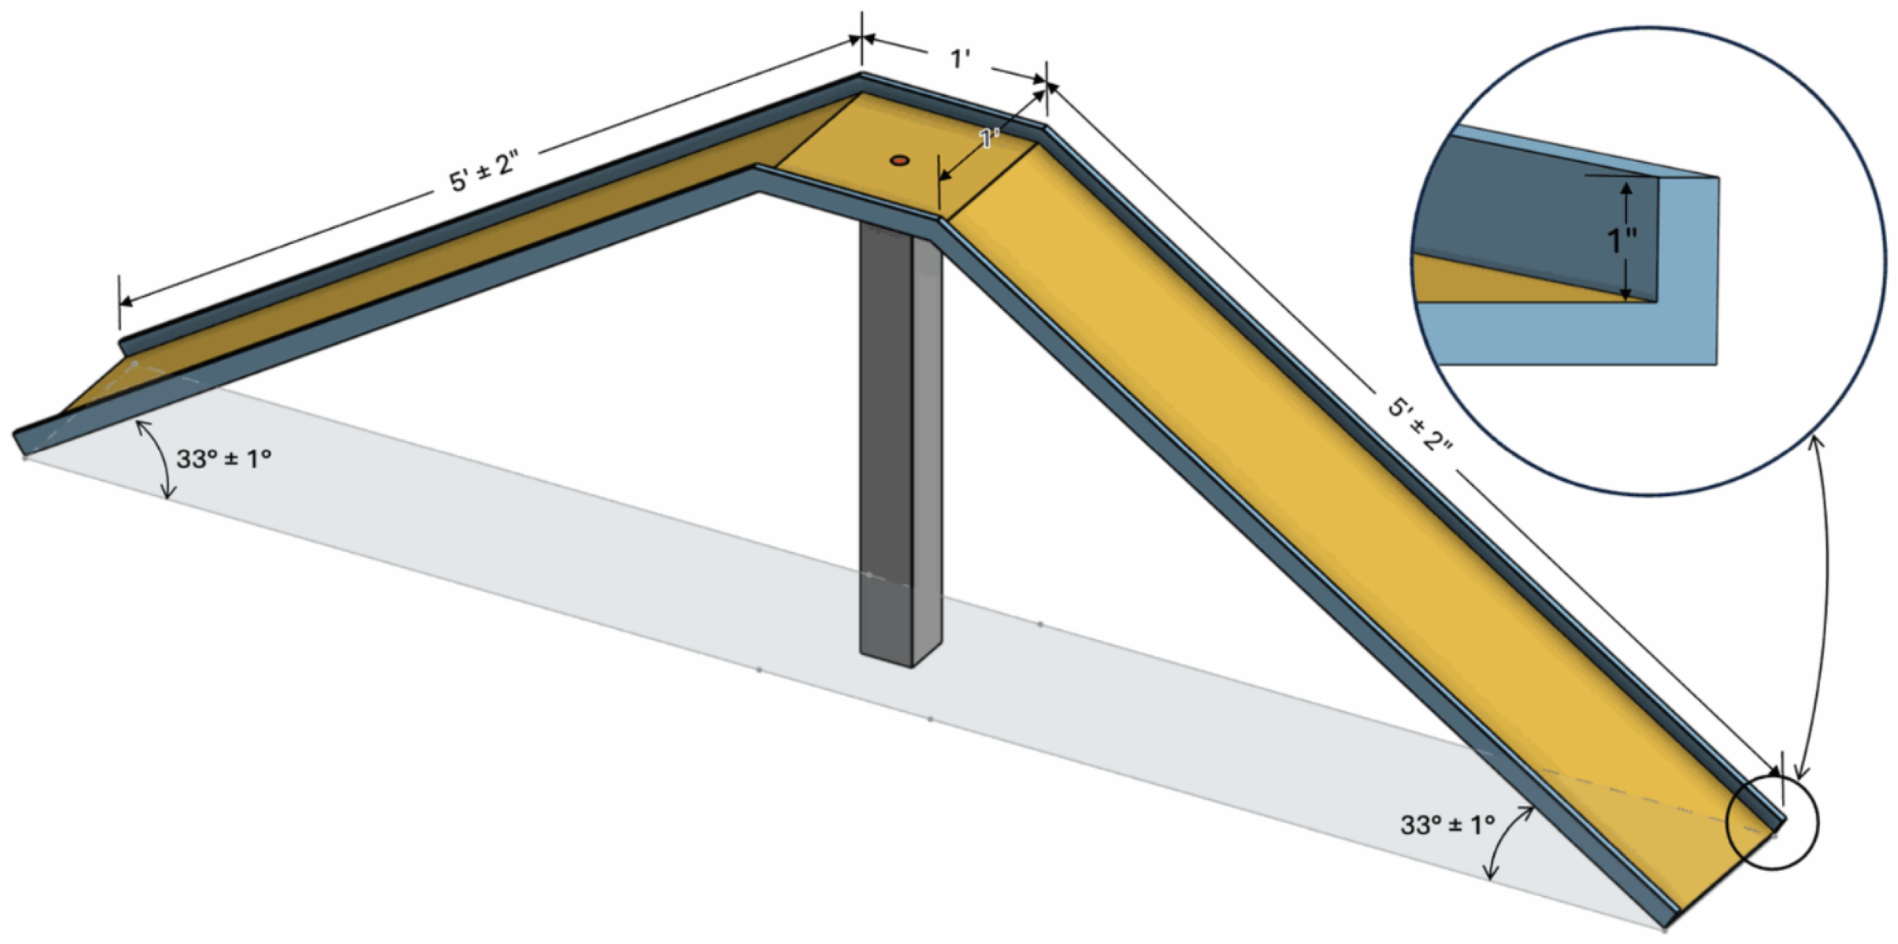
\includegraphics[width=0.85\textwidth]{fig01_hill.png}
  \caption{The contest hill. (a) Drawing from the course notes~\cite{ronney}. (b) Side view, to scale, with a robot on each ramp inside the \qty{12}{in} start zone.}
  \label{fig:hill}
\end{figure}

\subsection{Objective and strategy}
\label{sec:strategy}

Our objective was to reach the mesa first and keep the opponent from displacing us for the rest of the \qty{30}{s}. The lecture notes put it as ``possession is 9/10 of the law''~\cite{ronney}. The hill's geometry makes this even stronger. An attacker is still on the slope, fighting gravity, while the defender sits on the flat. And an attacker's wedge cannot sit flush until the robot has fully cleared the ramp, so its edge is still in the air at the moment it meets the defender.

Arriving first matters even more for an autonomous robot than for a driven one. Until the robots meet, the world is fully known: a \ang{33.4} slope of known length, then a flat mesa. After contact, a robot without vision cannot tell whether it is being pushed, lifted or turned, and ultrasonic range sensors are easy to confuse. A robot that is already on top needs very little information to hold its place.

The physics favors the defender too. On the flat mesa a robot can resist with its whole friction force, $\mu_s m g$. An attacker still on the ramp spends most of its traction holding itself on the slope and has only $\mu_s m g \cos\theta - m g \sin\theta$ left to push with. For two robots of equal mass and any $\mu_s$ between 0.8 and 1.0, the defender can resist 3.5 to 7 times the force the attacker can apply.

\paragraph{Defense without a pushing match}
Instead of planning to out-push an opponent, we put a low wedge with forks at the front of the robot, so an opponent arriving at the mesa edge drives up onto it and over or off the side. The forks are shaped to sit flush on the mesa even while the rest of the robot is still clearing the ramp (Section~\ref{sec:wedge}), so we never arrive with a raised edge ourselves. The stock kit robots have a flat polycarbonate bottom about 2 to \qty{3}{in} off the ground, which a low wedge slides under easily. \tbd{Confirm how sitting under an opponent scores under the farthest-point rule; our final match (Section~\ref{sec:results}) shows it can lose.}

\paragraph{The side wall as a guide rail}
The whole contest is a straight line, so the robot never has to turn. It does have to stay aligned: run straight up the ramp, not ride over the edge, and not waste energy scrubbing sideways. Running with one side against a guide rail does this mechanically, and side guards keep the robot from riding up over the rail (Section~\ref{sec:layout}).

These goals set four requirements that organize the rest of the report: climb as fast as traction and power allow, recognize the crest and stop at the front of the mesa, hold position there, and never depend on winning a sustained pushing match.

\section{Design concepts and selection}
\label{sec:concepts}

We considered only a handful of alternatives, and dropped each of them quickly. A hinged wedge, passive or spring-loaded, would have kept the wedge edge on the ramp surface, but fixed forks do the same job more simply and better (Section~\ref{sec:wedge}). A servo linkage bracing against both walls, and a side lifter to tip an opponent over the guide rail, were both too complex for the time we had, and an autonomous robot has no good way to know when to fire a lifter. Tennis grip tape on the tracks would have raised traction, but it slipped off because of the angle the tracks sit at (Section~\ref{sec:traction}).

What we built is a tracked robot with a forks-and-wedge front end that runs along a guide rail (Fig.~\ref{fig:robot}). The front end has no moving parts: on the mesa it turns an opponent's own drive force into the thing that removes it.

\begin{figure}[htbp]
  \centering
  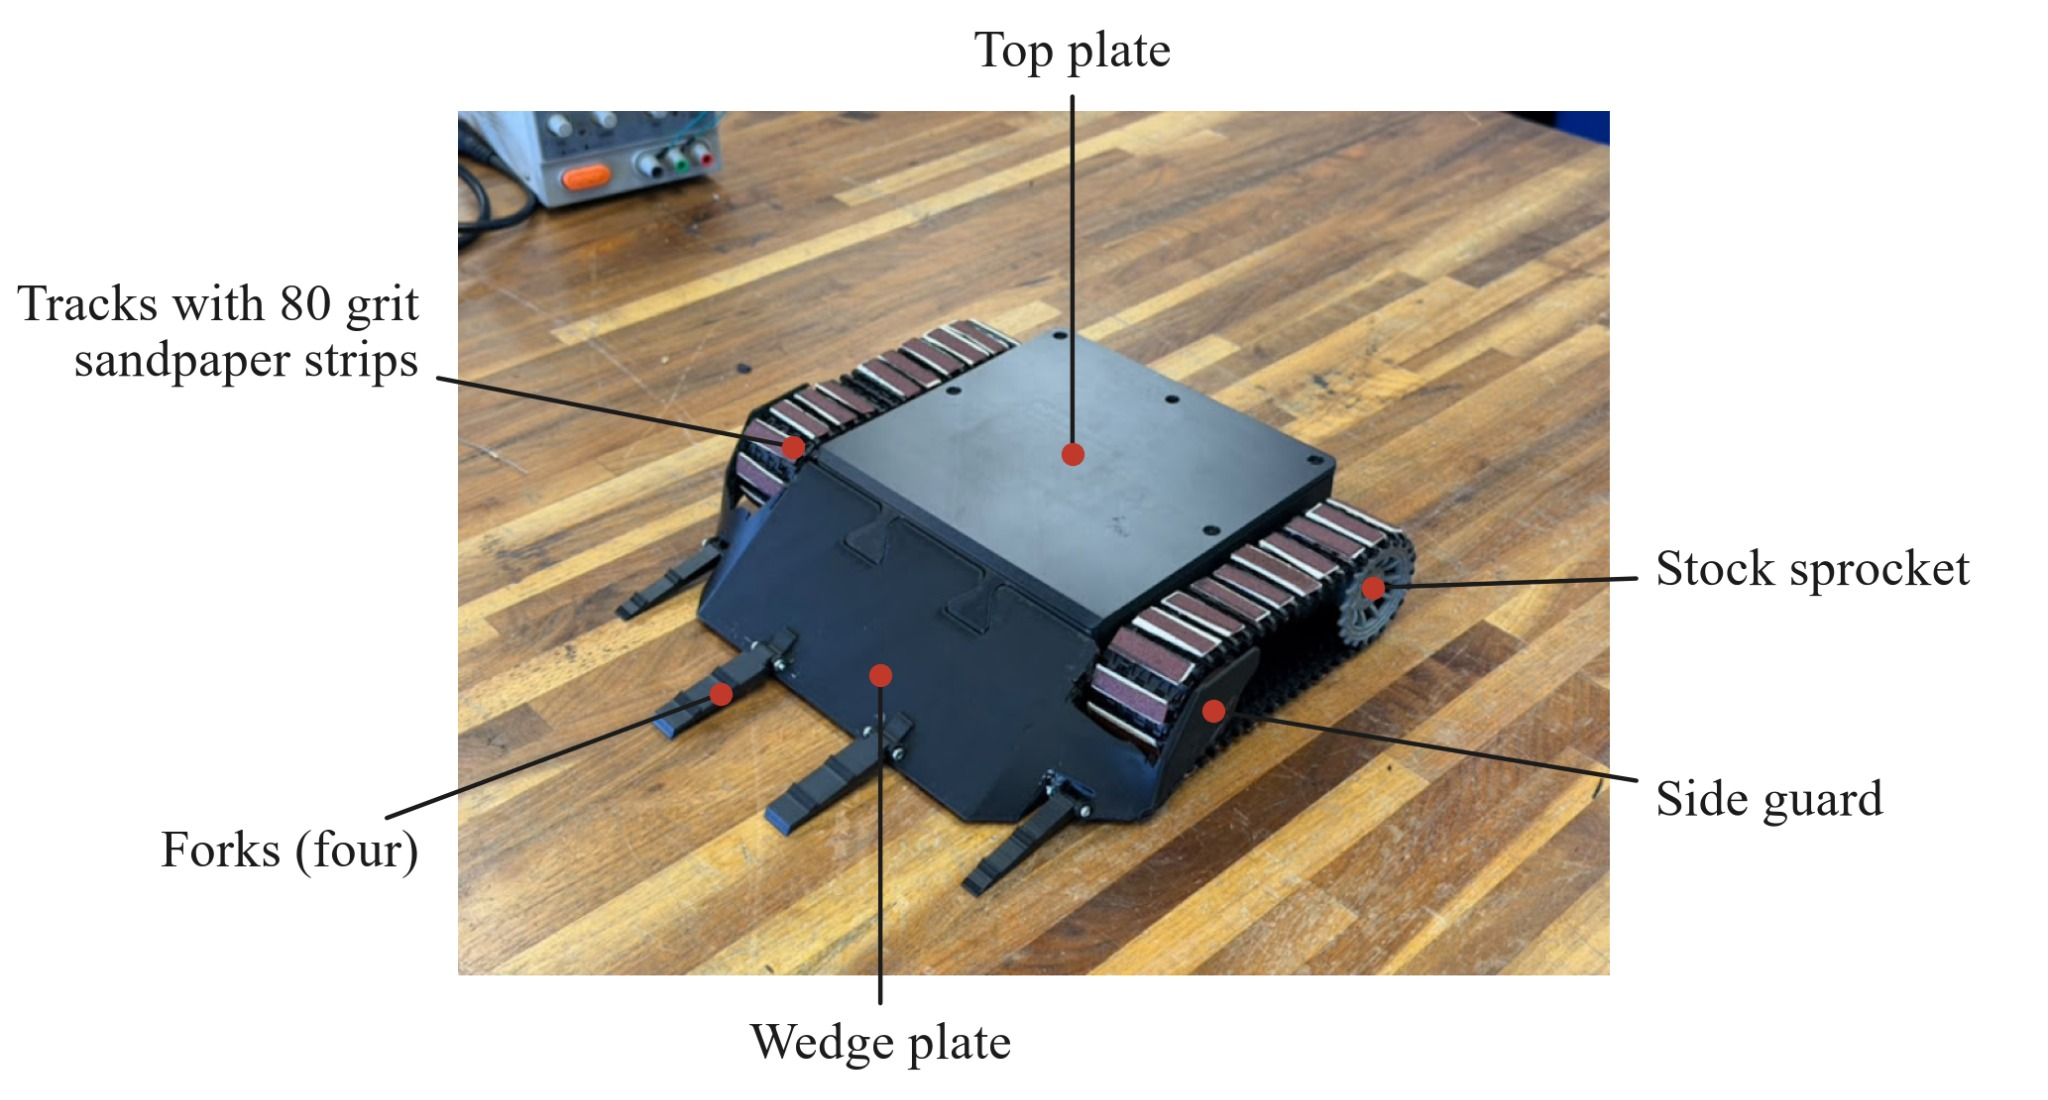
\includegraphics[width=\textwidth]{fig02_robot.jpg}
  \caption{The robot as built. A low wedge plate with four forks leads, the tracks carry strips of 80 grit sandpaper, and side guards run along each side.}
  \label{fig:robot}
\end{figure}

\section{Drivetrain}
\label{sec:drivetrain}

The drivetrain has to carry a \qty{0.97}{kg} robot up the \ang{33.4} slope as fast as possible. The kit motors were too slow for that, so we bought inexpensive gearmotors. We chose them by first bounding the options with three physical limits: the traction the tracks can transmit (Section~\ref{sec:traction-bound}), the force needed to climb (Section~\ref{sec:holding-bound}) and the current the electronics can supply (Section~\ref{sec:current-bound}). We then picked the gear ratio with the shortest predicted climb among the motors left (Section~\ref{sec:gear-ratio}).

\subsection{Upper bound on torque: traction}
\label{sec:traction-bound}

The tracks can push along the ramp only until they slip, at the static friction force $F_f$ (Fig.~\ref{fig:fbd}). The total drive force $F$ is therefore capped by the maximum available traction:
\begin{equation}
  F \le \mu_s N
  \label{eq:traction}
\end{equation}
where the normal force is $N = m g \cos\ang{33.4}$ on the ramp and $N = m g$ on the mesa. Each motor drives one track through a sprocket of \qty{50}{mm} diameter ($r = \qty{25}{mm}$) and supplies half of $F$, so the torque per motor at which the tracks start to slip is $\mu_s N r / 2$ at the sprocket. We estimated $\mu_s = 1.2$ to be the most any tread material on the ramp could reasonably give, since that is about the highest static friction coefficient that surfaces engineered for grip, such as tires, reach. On the ramp the maximum available traction is then \qty{9.5}{N}, and no motor can usefully deliver more than \qty{0.12}{N.m} at the sprocket (Table~\ref{tab:traction}).

\begin{figure}[htbp]
  \centering
  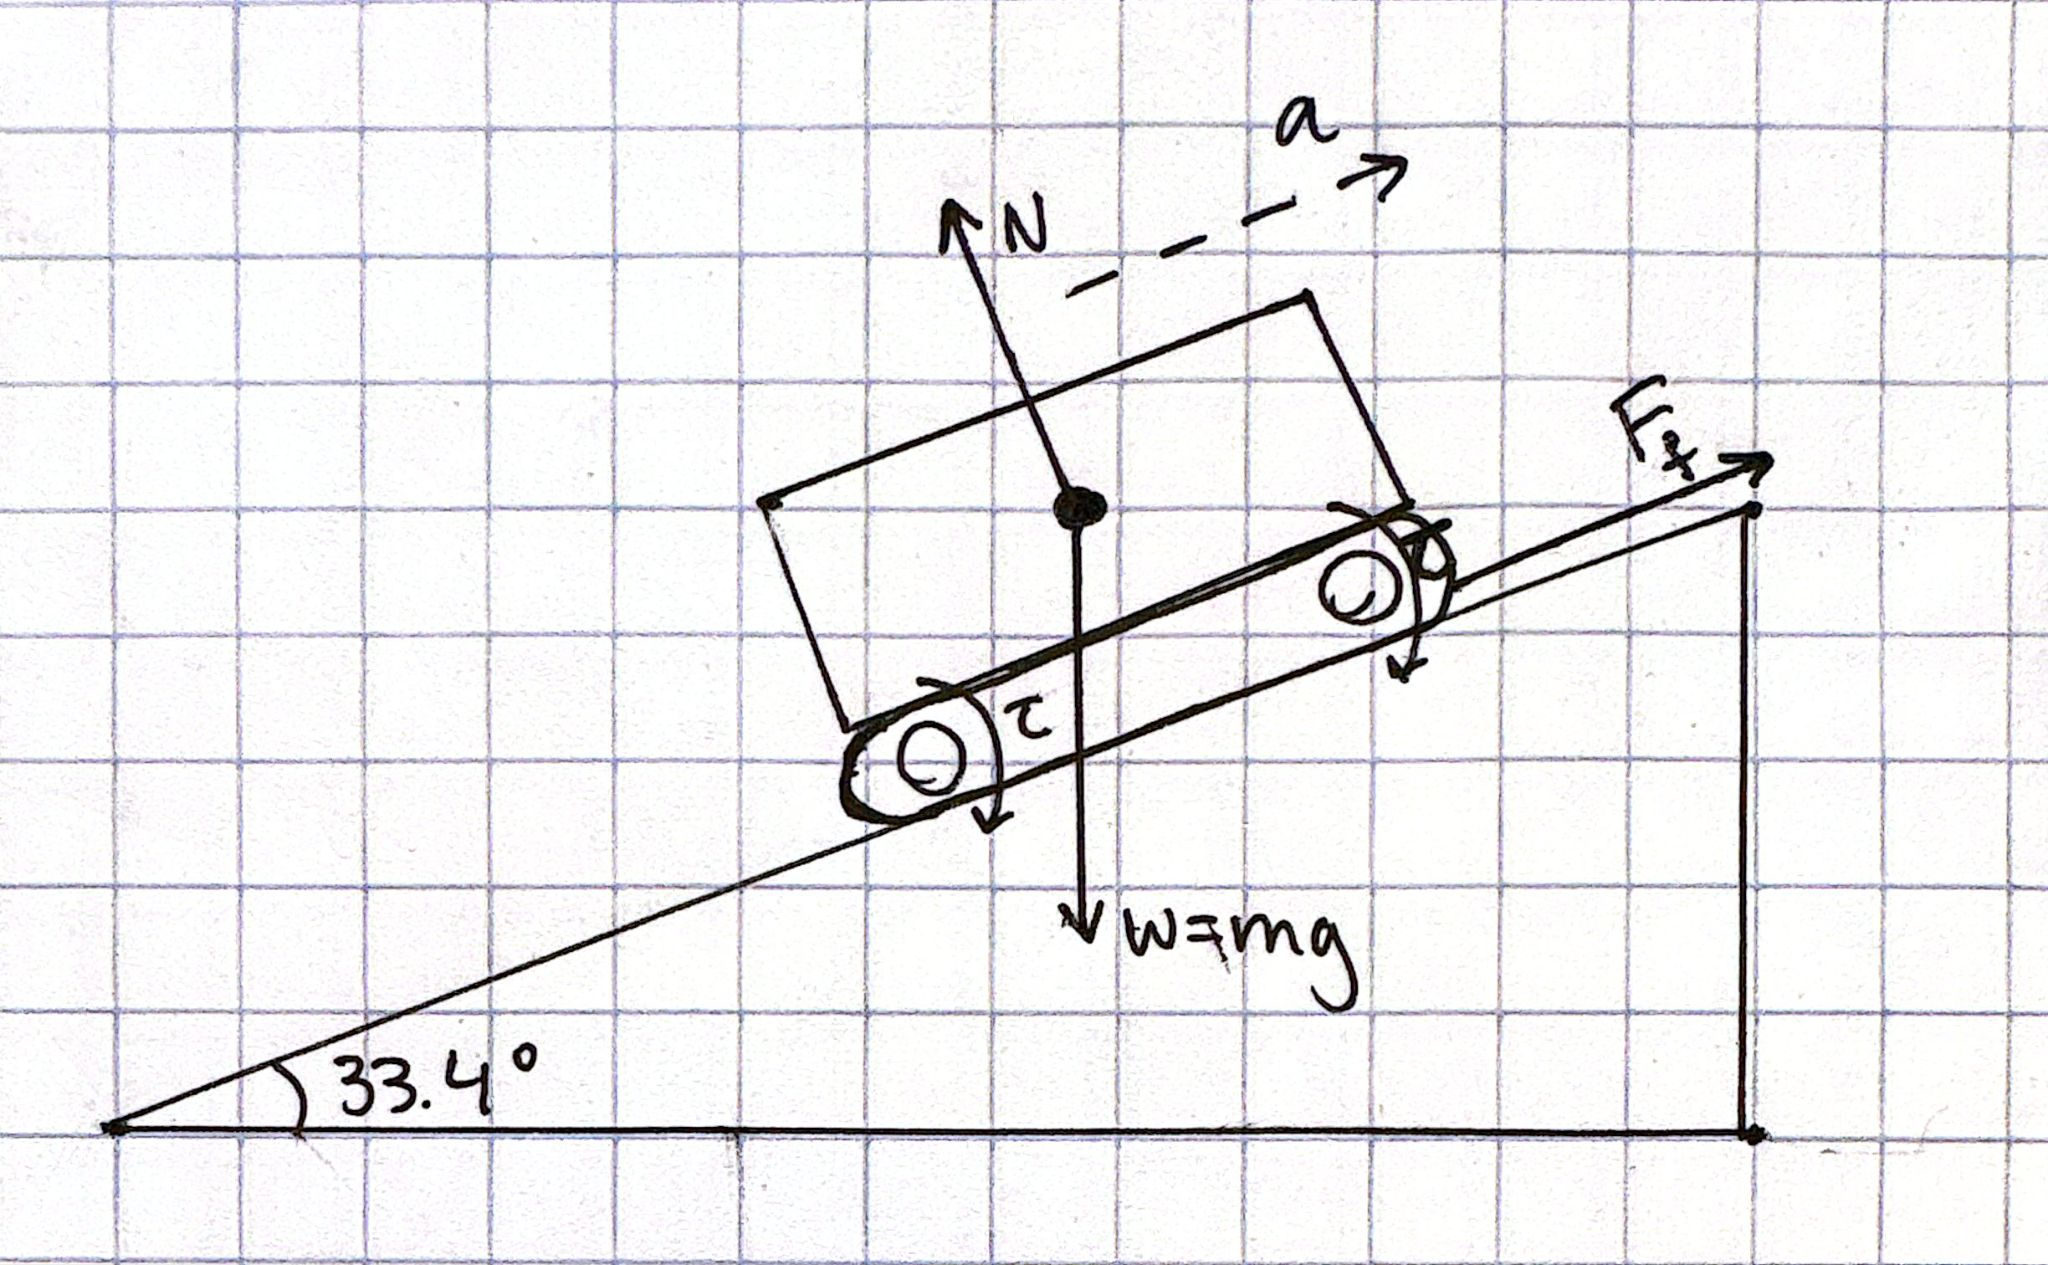
\includegraphics[width=0.58\textwidth]{fig03_fbd.jpg}
  \caption{Forces on the robot while it climbs. Friction at the tracks, $F_f$, is the only force pushing it up the ramp.}
  \label{fig:fbd}
\end{figure}

A real drivetrain also loses torque to resistance in the tracks, axles and couplers (Section~\ref{sec:holding-bound}), and we could not calculate how much before the drivetrain was built. The motors must supply that loss on top of the force the tracks transmit, so we allowed stall force up to three times the maximum available traction. The factor of 3 is a judgment call, generous on purpose because the losses were unknown. Physically, it means a motor at this bound could lose two thirds of its stall force inside the drivetrain and still deliver the full maximum available traction at stall. Excess stall force is not wasted outright: a motor's force falls as it speeds up (Eq.~\eqref{eq:motor}), so it only makes the tracks slip for the first part of the climb.

\begin{table}[htbp]
  \centering
  \caption{The most force the tracks of a \qty{0.97}{kg} robot can transmit before slipping (maximum available traction), and the matching maximum usable torque per motor at a \qty{50}{mm} sprocket, for three assumed values of the maximum $\mu_s$.}
  \label{tab:traction}
  \begin{tabular}{@{}c cc cc@{}}
    \toprule
    & \multicolumn{2}{c}{Ramp} & \multicolumn{2}{c}{Mesa} \\
    \cmidrule(lr){2-3}\cmidrule(l){4-5}
    Assumed & Max.\ static & Max.\ usable torque & Max.\ static & Max.\ usable torque \\
    maximum $\mu_s$ & friction force (\unit{N}) & per motor (\unit{N.m}) & friction force (\unit{N}) & per motor (\unit{N.m}) \\
    \midrule
    0.8 & 6.36 & 0.079 & 7.61  & 0.095 \\
    1.0 & 7.94 & 0.099 & 9.52  & 0.119 \\
    1.2 & 9.53 & 0.119 & 11.42 & 0.143 \\
    \bottomrule
  \end{tabular}
\end{table}

\subsection{Lower bound on torque: holding on the slope}
\label{sec:holding-bound}

Gravity pulls the robot down the ramp with $m g \sin\ang{33.4} = \qty{5.24}{N}$. To start from rest and climb, the motors' stall force must exceed that pull plus every other resistance:
\begin{equation}
  F_\mathrm{stall} > k_r\, m g \sin\ang{33.4}
  \label{eq:holding}
\end{equation}
Here $k_r$ is the total resistance to climbing as a multiple of gravity's pull, so $k_r - 1$, which we call the extra resistance, counts every resistance besides gravity and the gearbox losses, which Section~\ref{sec:gear-ratio} counts separately as the gearbox efficiency $\eta_\mathrm{g}$. A value of $k_r = 1$ would be a robot with no extra resistance; $k_r = 1.25$ means the extra resistance adds a quarter of gravity's pull, \qty{1.31}{N}. We could not calculate $k_r$ from first principles, because it comes from friction and deflection throughout the drivetrain and from rubbing on the side wall (Section~\ref{sec:drivetrain-result}). A motor that only just clears Eq.~\eqref{eq:holding} climbs, but with so little force to spare for acceleration it never reaches its full speed on a \qty{1.524}{m} ramp.

\subsection{Upper bound on motor size: current}
\label{sec:current-bound}

A bigger motor makes more power only by drawing more current. A brushed DC motor with winding resistance $R_\mathrm{w}$ stalls at $I_\mathrm{stall} = V / R_\mathrm{w}$ and delivers its peak mechanical power at half its stall torque and half its no-load speed:
\begin{equation}
  P_\mathrm{max} = \frac{V I_\mathrm{stall}}{4}
  \label{eq:pmax}
\end{equation}
The voltage is fixed by the kit's 2S pack, so stall current is a proxy for motor size: the largest viable motors are those whose current the electronics can supply. The motors will stall briefly at the start of every climb and could stall for a long time in a pushing match. Two components limit $I_\mathrm{stall}$ (Table~\ref{tab:current}).

\paragraph{Driver}
The TB6612FNG driver we had on hand is rated for \qty{1.2}{A} continuous and \qty{3.2}{A} peak per channel~\cite{tb6612}. A continuous stall, though unlikely, could occur in a pushing match, which caps $I_\mathrm{stall}$ at \qty{1.2}{A} per motor. Because most stalls are brief, up to \qty{3.2}{A} is acceptable.

\paragraph{Pack}
The 7805 linear regulator steps an input between 7 and \qty{25}{V} down to the \qty{5}{V} the Photon runs on~\cite{reg7805}. Below \qty{7}{V} input, the \qty{5}{V} supply cannot be held and the Photon behaves erratically or cuts out, which loses the match. The voltage sag from the motors in a likely worst case therefore must not pull the pack below \qty{7}{V}. The terminal voltage of a battery with open-circuit voltage $\mathcal{E}$ and internal resistance $R_\mathrm{int}$ is
\begin{equation}
  V_\mathrm{term} = \mathcal{E} - I_\mathrm{pack} R_\mathrm{int}
  \label{eq:vterm}
\end{equation}
so with both motors at stall the pack sags by $\Delta V_\mathrm{sag} = 2 I_\mathrm{stall} R_\mathrm{int}$, and the largest stall current per motor that keeps the pack above \qty{7}{V} is
\begin{equation}
  I_\mathrm{stall,max} = \frac{\mathcal{E} - \qty{7}{V}}{2 R_\mathrm{int}}
  \label{eq:istall-max}
\end{equation}
Taking $R_\mathrm{int} \approx \qty{0.15}{\ohm}$ \tbd{replace with our measured value from the voltage-drop test} and $\mathcal{E} = \qty{7.4}{V}$, Eq.~\eqref{eq:istall-max} gives $I_\mathrm{stall,max} = \qty{1.3}{A}$. The value \qty{7.4}{V} is the nominal 2S voltage; a 2S pack runs from \qty{8.4}{V} full to a usual cutoff of \qty{6.0}{V}~\cite{cell}. But even with both motors stalled throughout, six \qty{30}{s} runs draw only about \qty{0.14}{A.h}, a few percent of the pack's capacity, so the pack stays near nominal. The best case, a full pack at $\mathcal{E} = \qty{8.4}{V}$, allows \qty{4.7}{A} per motor.

\begin{table}[htbp]
  \centering
  \caption{Limits on the stall current of each motor, $I_\mathrm{stall}$, from the driver and from the pack.}
  \label{tab:current}
  \begin{tabularx}{\textwidth}{@{}L L c L c@{}}
    \toprule
    & \multicolumn{2}{c}{Worst case} & \multicolumn{2}{c}{Best case} \\
    \cmidrule(lr){2-3}\cmidrule(l){4-5}
    Limiting component & Condition & Max.\ $I_\mathrm{stall}$ (\unit{A}) & Condition & Max.\ $I_\mathrm{stall}$ (\unit{A}) \\
    \midrule
    Driver (TB6612FNG) & Stall held, as in a pushing match & 1.2 & Brief stall at the start of a climb & 3.2 \\
    Pack (7805 drops out below \qty{7.0}{V}) & Pack at \qty{7.4}{V} & 1.3 & Full pack at \qty{8.4}{V} & 4.7 \\
    \bottomrule
  \end{tabularx}
\end{table}

We wanted a motor wound for close to our pack voltage. The match does not have to be exact: above its rated voltage a motor's speed and stall current rise in proportion, so a \qty{6}{V} motor on our \qty{7.4}{V} pack runs about \qty{23}{\percent} faster and draws about \qty{23}{\percent} more current, which Table~\ref{tab:current} must allow. A \qty{37}{mm} gearmotor stalls at \qty{5.5}{A} even at its \qty{12}{V} rating~\cite{pololu37d}, several times our worst-case limit. Pololu's \qty{25}{mm}, \qty{6}{V} gearmotors stall at about \qty{2.0}{A}~\cite{pololu25d}. The cheaper \qty{25}{mm} motors we found on Amazon are rated at \qty{2.7}{W}~\cite{meccanixity}; taking that as the peak power on our pack, Eq.~\eqref{eq:pmax} gives $I_\mathrm{stall} = 4 P_\mathrm{max} / V = \qty{1.46}{A}$, about \qty{1.5}{A}. That is just above the worst-case limit and well inside the best case, so of the sizes we compared, a \qty{25}{mm} gearmotor wound for \qty{6}{V} fits the kit pack best.

\subsection{Choosing the gear ratio inside the bounds}
\label{sec:gear-ratio}

The listing offers \qty{25}{mm} \qty{6}{V} gearmotors with ratios from 1:4.4 to 1:500~\cite{meccanixity}. Changing the ratio on the same base motor only reallocates power between speed and torque. Too low a ratio gives too little torque to accelerate the robot against gravity and drivetrain resistance. Too high a ratio wastes gearing on torque the tracks cannot use and limits top speed. To find the optimum, we wrote the estimated climb time as a function of gear ratio, $t_\mathrm{climb}(G)$, and evaluated it for every version on sale.

\paragraph{Motor model}
A brushed DC motor makes torque in proportion to its current, and the pack voltage divides between the winding resistance and the back-EMF the spinning motor generates. In SI units the torque constant and the back-EMF constant are the same number, $k_\mathrm{t}$, so $\tau_\mathrm{m} = k_\mathrm{t} I_\mathrm{m}$ and $V = I_\mathrm{m} R_\mathrm{w} + k_\mathrm{t}\, \omega_\mathrm{m}$. Eliminating $I_\mathrm{m}$ shows torque falling linearly from its stall value to zero at the no-load speed. We had to choose before we had a motor to test, so we took the no-load speed from the listing, about \qty{6000}{\rpm} (\qty{625}{rad/s}) at \qty{6}{V}, and our estimated stall current of \qty{1.5}{A} on the \qty{7.4}{V} pack:
\begin{equation}
  k_\mathrm{t} = \frac{\qty{6}{V}}{\qty{625}{rad/s}} = \qty{0.0096}{N.m/A}, \qquad
  R_\mathrm{w} = \frac{\qty{7.4}{V}}{\qty{1.5}{A}} = \qty{4.9}{\ohm}
  \label{eq:k}
\end{equation}
The gearbox divides speed by $G$ and multiplies torque by $G$, losing a fraction of the torque to the gearbox efficiency $\eta_\mathrm{g}$, and the sprocket of radius $r$ turns shaft torque into track force. For both motors together, the drive force at robot speed $v$ is
\begin{equation}
  F(v) = F_\mathrm{stall}\left(1 - \frac{v}{v_0}\right), \qquad
  F_\mathrm{stall} = \frac{2 \eta_\mathrm{g} k_\mathrm{t} G V}{R_\mathrm{w} r}, \qquad
  v_0 = \frac{V r}{k_\mathrm{t} G}
  \label{eq:motor}
\end{equation}
Raising $G$ raises $F_\mathrm{stall}$ and lowers $v_0$ in the same proportion.

\paragraph{Equation of motion}
Two kinds of resistance oppose the drive force. Internal losses eat motor torque before it reaches the ramp: friction within the treads, the side guards rubbing on the treads, and the energy spent flexing the couplers as they turn. External resistance acts on the robot directly, as gravity does: friction and small collisions against the side wall. We lump both into $k_r$ (Eq.~\eqref{eq:holding}), so the total resistance is $F_\mathrm{r} = k_r\, m g \sin\ang{33.4}$. The drive force also cannot exceed the maximum available traction, $\mu_s m g \cos\ang{33.4}$ (Eq.~\eqref{eq:traction}); for $t_\mathrm{climb}(G)$ we took $\mu_s = 1.0$, the middle row of Table~\ref{tab:traction}. Newton's second law along the ramp is then
\begin{equation}
  m \frac{dv}{dt} = \min\!\left[F(v),\ \mu_s m g \cos\ang{33.4}\right] - F_\mathrm{r}
  \label{eq:climb}
\end{equation}
Gear losses grow with the load, so $\eta_\mathrm{g}$ scales the motor force, while $k_r$ is a constant drag. Subtracting internal losses after capping the drive force overstates them while the tracks slip, so the model errs slow, and it assumes full motor duty from the start.

\paragraph{Solving for the climb time}
$t_\mathrm{climb}(G)$ is the time Eq.~\eqref{eq:climb}, started from rest, takes to carry the robot \qty{1.524}{m}. The minimum splits the climb into two phases. At low speed the tracks slip and the robot accelerates uniformly at the traction limit; for the \qty{280}{\rpm} version this lasts \qty{0.17}{s} and covers \qty{4}{cm}. After that the motors limit the force, Eq.~\eqref{eq:climb} becomes linear, and the speed approaches exponentially the speed $v_t = v_0(1 - F_\mathrm{r}/F_\mathrm{stall})$ at which drive force balances resistance, with time constant $t_0 = m v_0 / F_\mathrm{stall} = \qty{0.05}{s}$. We integrated once more for position and found the time to cover \qty{1.524}{m} by bisection.

\paragraph{Why there is an optimum}
The robot spends nearly the whole climb close to $v_t$ (\qty{0.63}{m/s} for the \qty{280}{\rpm} version with $\eta_\mathrm{g} = 0.7$ and $k_r = 1$), so the fastest climb comes from the largest $v_t$. Substituting the stall force and no-load speed into $v_t$ and setting its derivative with respect to $G$ to zero, $v_t$ is largest when
\begin{equation}
  F_\mathrm{stall} = 2 F_\mathrm{r}
  \label{eq:optimum}
\end{equation}
At that gear ratio the motors climb at half their no-load speed, where a DC motor delivers its peak power. More reduction makes the motors strong but slow. Less reduction leaves so little force to spare over $F_\mathrm{r}$ that the motors must run close to stall to keep climbing. For the three combinations of $\eta_\mathrm{g}$ and $k_r$ in Fig.~\ref{fig:gear}b, Eq.~\eqref{eq:optimum} puts the optimum between the \qty{620}{\rpm} (1:9.6) and \qty{280}{\rpm} (1:21.3) versions.

\paragraph{Applying the bounds}
Every version shares the same base motor, so all of them meet Section~\ref{sec:current-bound}. The torque bounds of Sections~\ref{sec:traction-bound} and~\ref{sec:holding-bound} leave three candidates: the 170, 280 and \qty{620}{\rpm} versions (Fig.~\ref{fig:gear}a). The \qty{280}{\rpm} version (1:21.3) gives the shortest estimated climb (Fig.~\ref{fig:gear}b). It stays fastest for every combination of $\eta_\mathrm{g}$ from 0.5 to 0.8 and $k_r$ from 1.0 to 1.25 except the most optimistic corner, $\eta_\mathrm{g}$ of 0.75 or more with $k_r$ of about 1.1 or less, where the \qty{620}{\rpm} version is slightly faster. Nothing is sold between 280 and \qty{620}{\rpm}.

\begin{figure}[htbp]
  \centering
  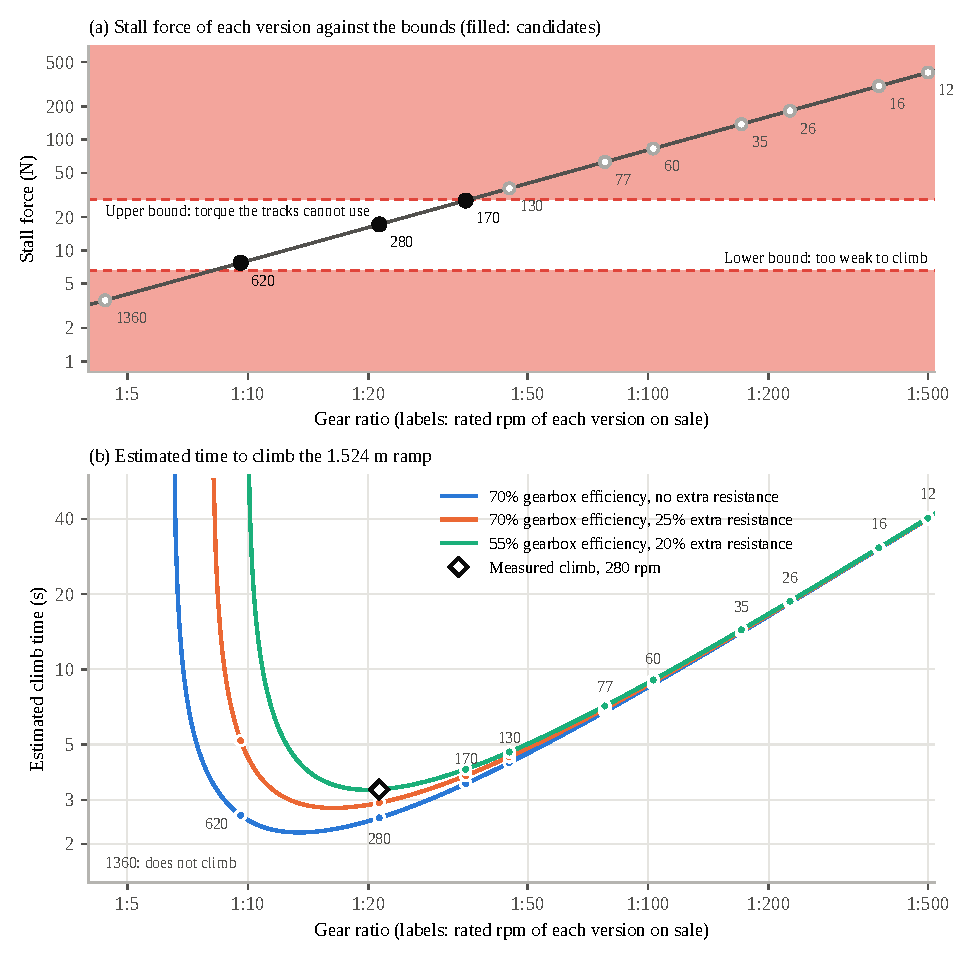
\includegraphics[width=0.74\textwidth]{fig04_gear_ratio.pdf}
  \caption{Choosing the gear ratio. (a) Stall force of each version on the \qty{7.4}{V} pack ($\eta_\mathrm{g} = 0.7$). Only the 170, 280 and \qty{620}{\rpm} versions fall between the lower bound (Section~\ref{sec:holding-bound}) and the upper bound (Section~\ref{sec:traction-bound}). (b) Estimated climb time $t_\mathrm{climb}(G)$ from Eq.~\eqref{eq:climb}. The \qty{280}{\rpm} version is fastest in all three cases, and our measured \qty{3.3}{s} climb falls on the curve for \qty{55}{\percent} gearbox efficiency with \qty{20}{\percent} extra resistance.}
  \label{fig:gear}
\end{figure}

\subsection{Result}
\label{sec:drivetrain-result}

We bought and ran the \qty{280}{\rpm} version. We measured its stall current on a charged pack at \qty{1.4}{A}, close to the \qty{1.5}{A} we had estimated. In three stopwatch trials the robot climbed the ramp in about \qty{3.3}{s}. For the \qty{280}{\rpm} version, $t_\mathrm{climb}(G)$ gives 2.4 to \qty{3.8}{s} over our range of losses, $\eta_\mathrm{g}$ from 0.5 to 0.8 and $k_r$ from 1.0 to 1.25, and \qty{2.5}{s} with no extra resistance ($\eta_\mathrm{g} = 0.7$, $k_r = 1$). The measured time falls inside that range, so the model is consistent with the measurement. One climb time cannot separate the two losses: $\eta_\mathrm{g} = 0.55$ with $k_r = 1.2$, for example, gives \qty{3.3}{s}.

Several problems in our build add to that resistance. The side guards flexed into the treads and rubbed on them in every run (Section~\ref{sec:layout}). The tracks are tensioned tightly so they do not dip and scrape at the mesa edge (Section~\ref{sec:couplers}), which loads the sprockets and axles. The printed couplers flex as they turn, the treads have friction within themselves, and the robot rubs and knocks against the side wall it uses as a guide rail.

\section{Traction}
\label{sec:traction}

Section~\ref{sec:drivetrain} showed that traction caps how much of the motors' torque the robot can use, so the track surface is the most leveraged part of the drivetrain.

The stock tracks are hard plastic links: they provide almost no friction, and using them, our robot was unable to climb at all. The final surface is strips of 80 grit sandpaper taped onto the stock tracks (Fig.~\ref{fig:tracks}).

\begin{figure}[htbp]
  \centering
  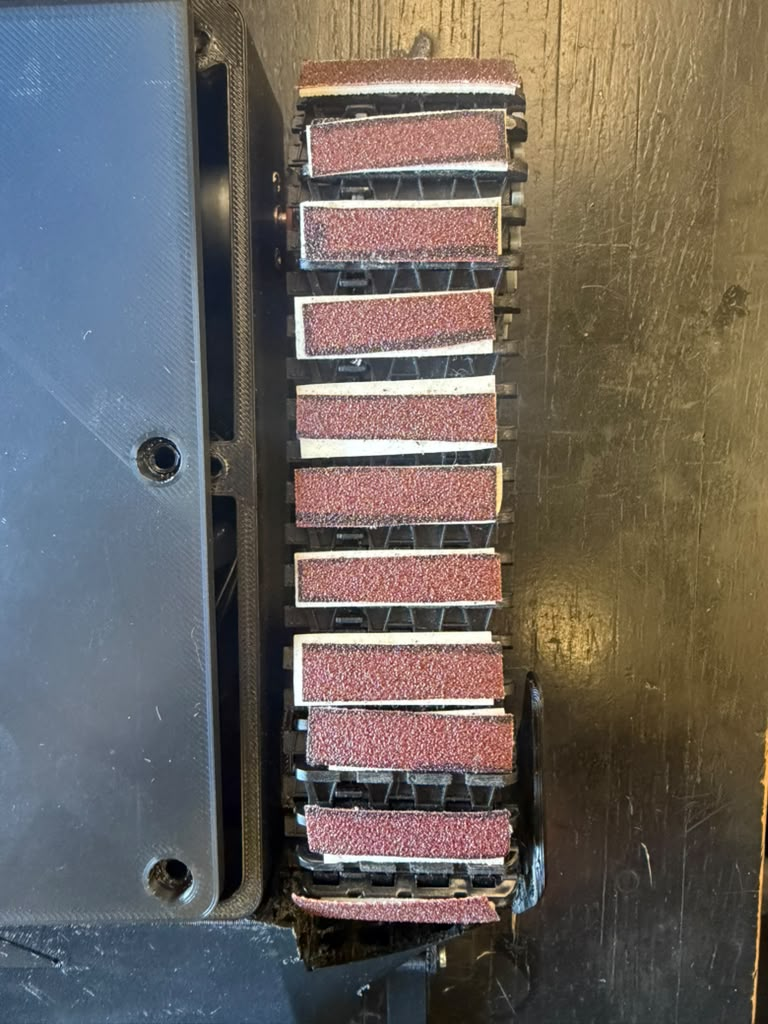
\includegraphics[width=0.34\textwidth]{fig05_tracks.jpg}
  \caption{\tbd{Caption.}}
  \label{fig:tracks}
\end{figure}

% we haven't done this - if we don't ever end up doing this we need a backup plan
To measure $\mu_s$ we \tbd{placed the robot on the ramp surface and raised the angle until it slipped, so \mbox{$\mu_s = \tan\theta_\mathrm{slip}$}; or pulled it with a luggage scale until it slid, so \mbox{$\mu_s = F/N$}}. We tested each surface \tbd{three times at each of three normal forces, adding \_\_\_ g of mass between sets} (Table~\ref{tab:friction}).

\begin{table}[htbp]
  \centering
  \caption{Measured static friction coefficients.}
  \label{tab:friction}
  \begin{tabular}{@{}l c c c c c@{}}
    \toprule
    Surface & Normal force (\unit{N}) & Trial 1 & Trial 2 & Trial 3 & Mean $\mu_s$ \\
    \midrule
    Stock tracks & \tbd{\ } & \tbd{\ } & \tbd{\ } & \tbd{\ } & \tbd{\ } \\
    Stock tracks & \tbd{\ } & \tbd{\ } & \tbd{\ } & \tbd{\ } & \tbd{\ } \\
    Stock tracks & \tbd{\ } & \tbd{\ } & \tbd{\ } & \tbd{\ } & \tbd{\ } \\
    \midrule
    Sandpaper    & \tbd{\ } & \tbd{\ } & \tbd{\ } & \tbd{\ } & \tbd{\ } \\
    Sandpaper    & \tbd{\ } & \tbd{\ } & \tbd{\ } & \tbd{\ } & \tbd{\ } \\
    Sandpaper    & \tbd{\ } & \tbd{\ } & \tbd{\ } & \tbd{\ } & \tbd{\ } \\
    \bottomrule
  \end{tabular}
\end{table}

\tbd{Result: sandpaper raised \mbox{$\mu_s$} from \_\_\_ to \_\_\_, which by Eq.~\eqref{eq:traction} raises the most force the tracks can transmit on the ramp from \_\_\_ to \_\_\_ N.}

\section{Chassis, wedge, forks and side guards}
\label{sec:chassis}

\subsection{Layout and construction}
\label{sec:layout}

The chassis is fully custom and 3D printed in PLA (Figs.~\ref{fig:chassis} to~\ref{fig:dimensions}). The wedge plate and forks form the front of the chassis. The battery holder sits in the front half, with the breadboard carrying the controller, motor driver and sensors beside it. The two gearmotors sit at the rear, each driving a stock sprocket, and the start switch is on the side where the judge can reach it.

% I  wanat to redo this to also point at the slot that allows you to fit a ratcheting socket wrench in to adjust the undriven wheels, and only label a singlne gearmotor. Also we already labeled the wedge elsewhere so I don't want to be redundant.
\begin{figure}[htbp]
  \centering
  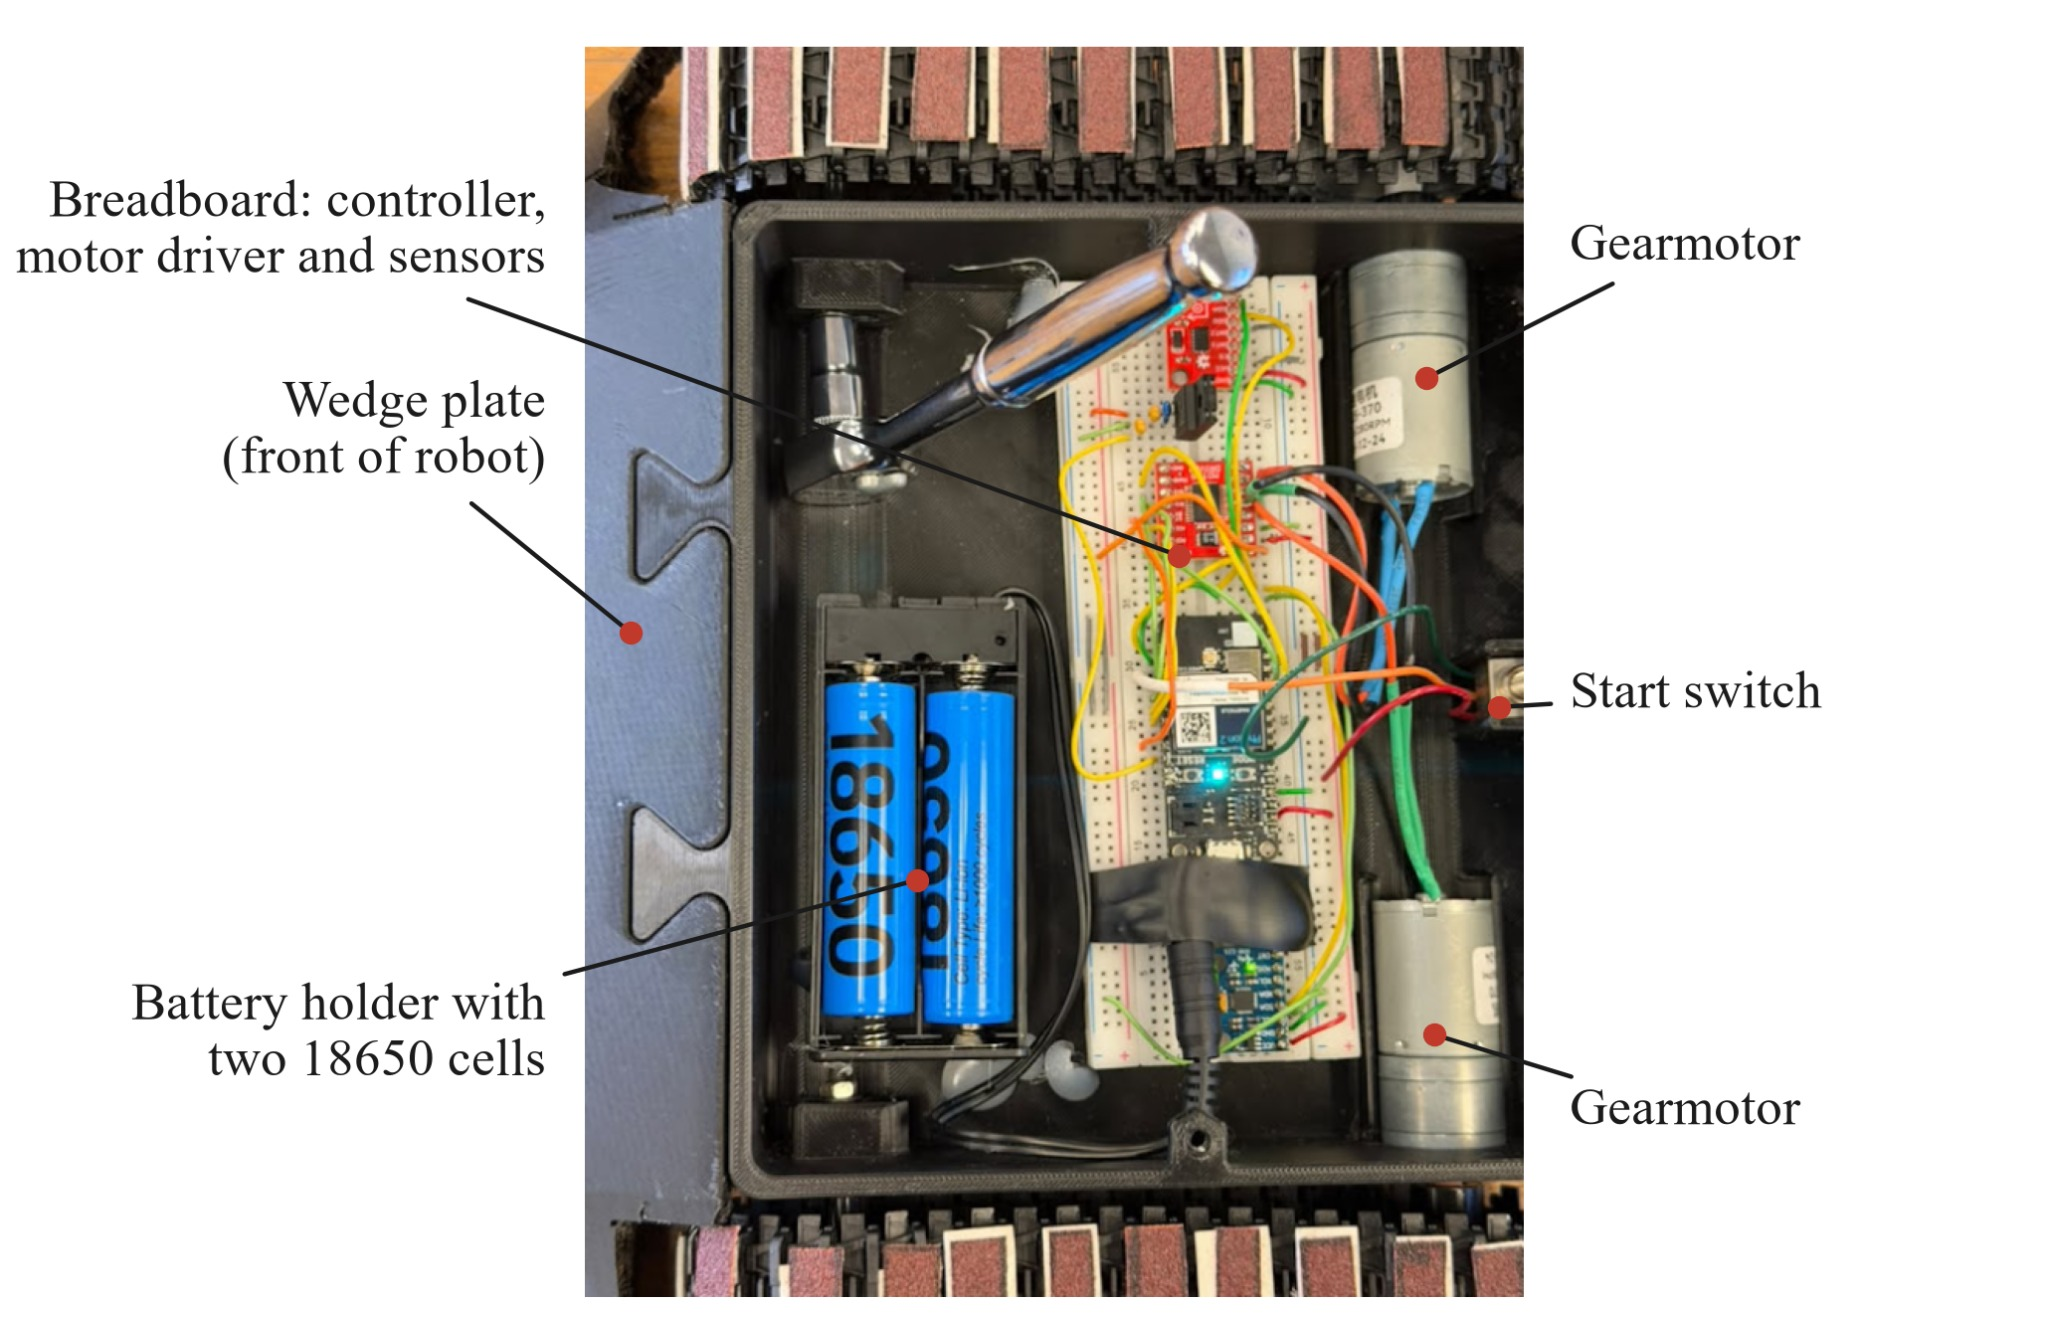
\includegraphics[width=\textwidth]{fig07_chassis.jpg}
  \caption{Inside the chassis with the top plate removed: the wedge plate at the front, the battery holder, the breadboard carrying the controller, motor driver and sensors, the two gearmotors and the start switch.}
  \label{fig:chassis}
\end{figure}

We used a master model workflow where key reference and control geometry flows down through all parts in the assembly. Our final design assembled from four parts: a main body enclosing the electronics, top plate, front wedge, and forks. We ran multiple test prints to check the battery box and board mounting patterns. However, in the final build we hot glued these parts for greater flexibility, which allowed us to change the configuration without reprinting the entire box.

We iterated a few drivetrain mounting prototypes. We realized that sufficient tread tension to prevent the robot from bottoming out on the ridge was crucial. However, to actually assemble then tense the treads would require the wheel pitch to be adjustable. So, we designed slots rather than clearance holes to mount the undriven wheel axle bolts. We also used slicer volume modifiers to raise the infill to 100\% where the bolt applies clamping stress to the plastic, ensuring we could tighten the axles to perfectly rigid with significant tension without the hollow plastic yielding.

Another crucial subassembly was the shaft coupler that adapted the 4mm male D-shaft of the motor to the 6mm female D-shaft of the sprocket. The coupler fits over the motor shaft and inserts into the sprocket shaft recess, fastened to the motor by a shaft collar and to the sprocket by a self-tapping screw that runs through the sprocket.

% if we can use this to guesstimate the positional tolerance of the printer that would be lit and a huge flex, boon to the testing side of thigns.
These required significant measurement, iteration, and testing to function correctly. The fit class between the coupler and each part it connects plays a significant role in how well it functions: too loose a fit (locational clearance) results in a shaft that sits at an angle when tensed with the tread.  It will gyrate and experience particularly particularly unfavorable strain cycles when spun. Too close a fit (interference) means it doesn't assemble. This part requires a running fit. Printing a sweep of different clearance values from 0.05mm to 0.15mm with a resolution of 0.05mm, we found the right clearance for the couplers to be 0.1mm.

Other iteration cycles also centered on clearances and tolerances. Insufficiently clearanced motor mounts and horizontal screw holes resulted in nonfunctional prototypes. After three test iterations, we settled on a mating interface clearance of 0.14mm for the motor mounts and horizontal screw holes.

We followed that up with a few isolated-drivetrain test prints to determine the necessary width for the undriven axle assembly slot such that it assembled easily, which needed to be almost doubled to 15mm from 8mm.

A full prototype chassis followed, then the shaft couplers and motor mounts. To further aid assembly, the top plate included drafted countersunk screw clearance holes and alignment ridges to guide the part into place.

The front wedge we designed as a unified part that wrapped the front of the robot, providing the wedge, side guards, and fork mounts. One difficult thing to design and optimize was the multi-part nature of the robot: manufacturing the entire thing at once wouldn't have been feasible in the build volume of my Prusa Core One+, so it took iteration to find the best places to split and reassemble. Originally, we had planned to print full-length side guards separately, but ditched the idea after realizing that the treads didn't need to be covered along the whole length of the robot. To preempt the need for additional fasteners or gluing, and leave modularity on the table, we designed the front wedge to mate to the rest of the chassis using dovetail joints with semi-permanent snsap fit nubs.
% I have good slicer screenshot for this that I want to include

The front wedge required careful design for printability in order to fit inside the available build volume. For a long, roughly linear part, available volume is maximized by approximately maximizing linear space (the diagonal). Therefore, we included a small 45 degree planar cutoff at the sides to print it at an angle, using tree supports both as supporting outriggers to prevent it from tipping over and to support overhangs.

A significant issue with our design was that the geometry that aimed to fully wrap and enclose the front surface of the treads assumed their nominal pitch of 120mm. However, our assembly procedure was designed to shove the treads as far forward as possible, and we failed to account for this in the design. This resulted in a 5mm interference on all sides between the front surface of the treads and the wedge. Without time to reprint, we used the bandsaw to chop out expanded clearances. This was one contributor to our low drivetrain efficiency, because the side guards were deprived of rigidity and frequently flexed into the treads. (Section~\ref{sec:drivetrain-result}).

At about \qty{4}{in} tall on an \qty{11.75}{in} by \qty{11.4}{in} footprint, the robot cannot tip backward on the \ang{33.4} ramp, and it never came close in testing.

% make this likea "Left: " and "Right: " syntax caption
% also your label for the right is wrong, the right is as a *section view* of the electronics box that cuts away so you can see the internal mounting components better
\begin{figure}[htbp]
  \centering
  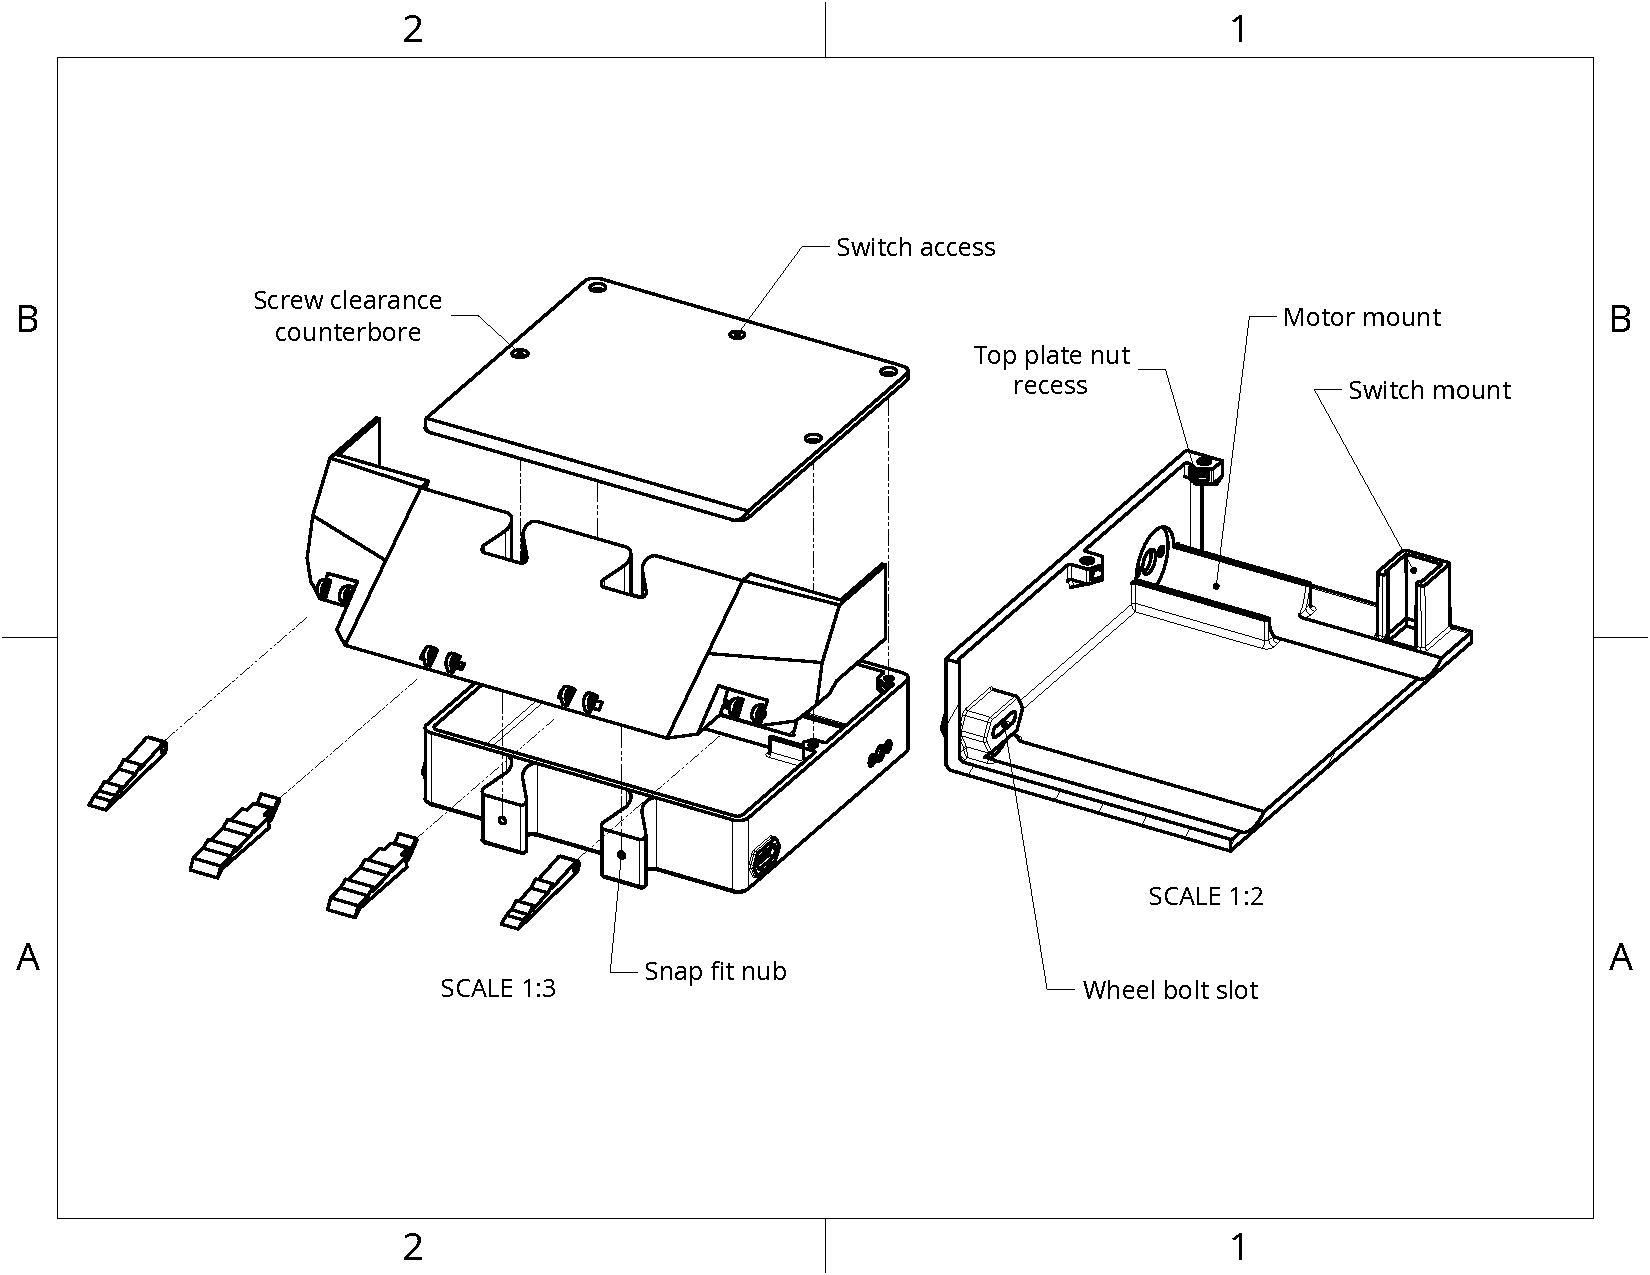
\includegraphics[width=0.8\textwidth]{fig_chassis_assembly.pdf}
  \caption{Exploded assembly drawing of the chassis (scale 1:3), with the base alone at right (scale 1:2).}
  \label{fig:assembly}
\end{figure}

\begin{figure}[htbp]
  \centering
  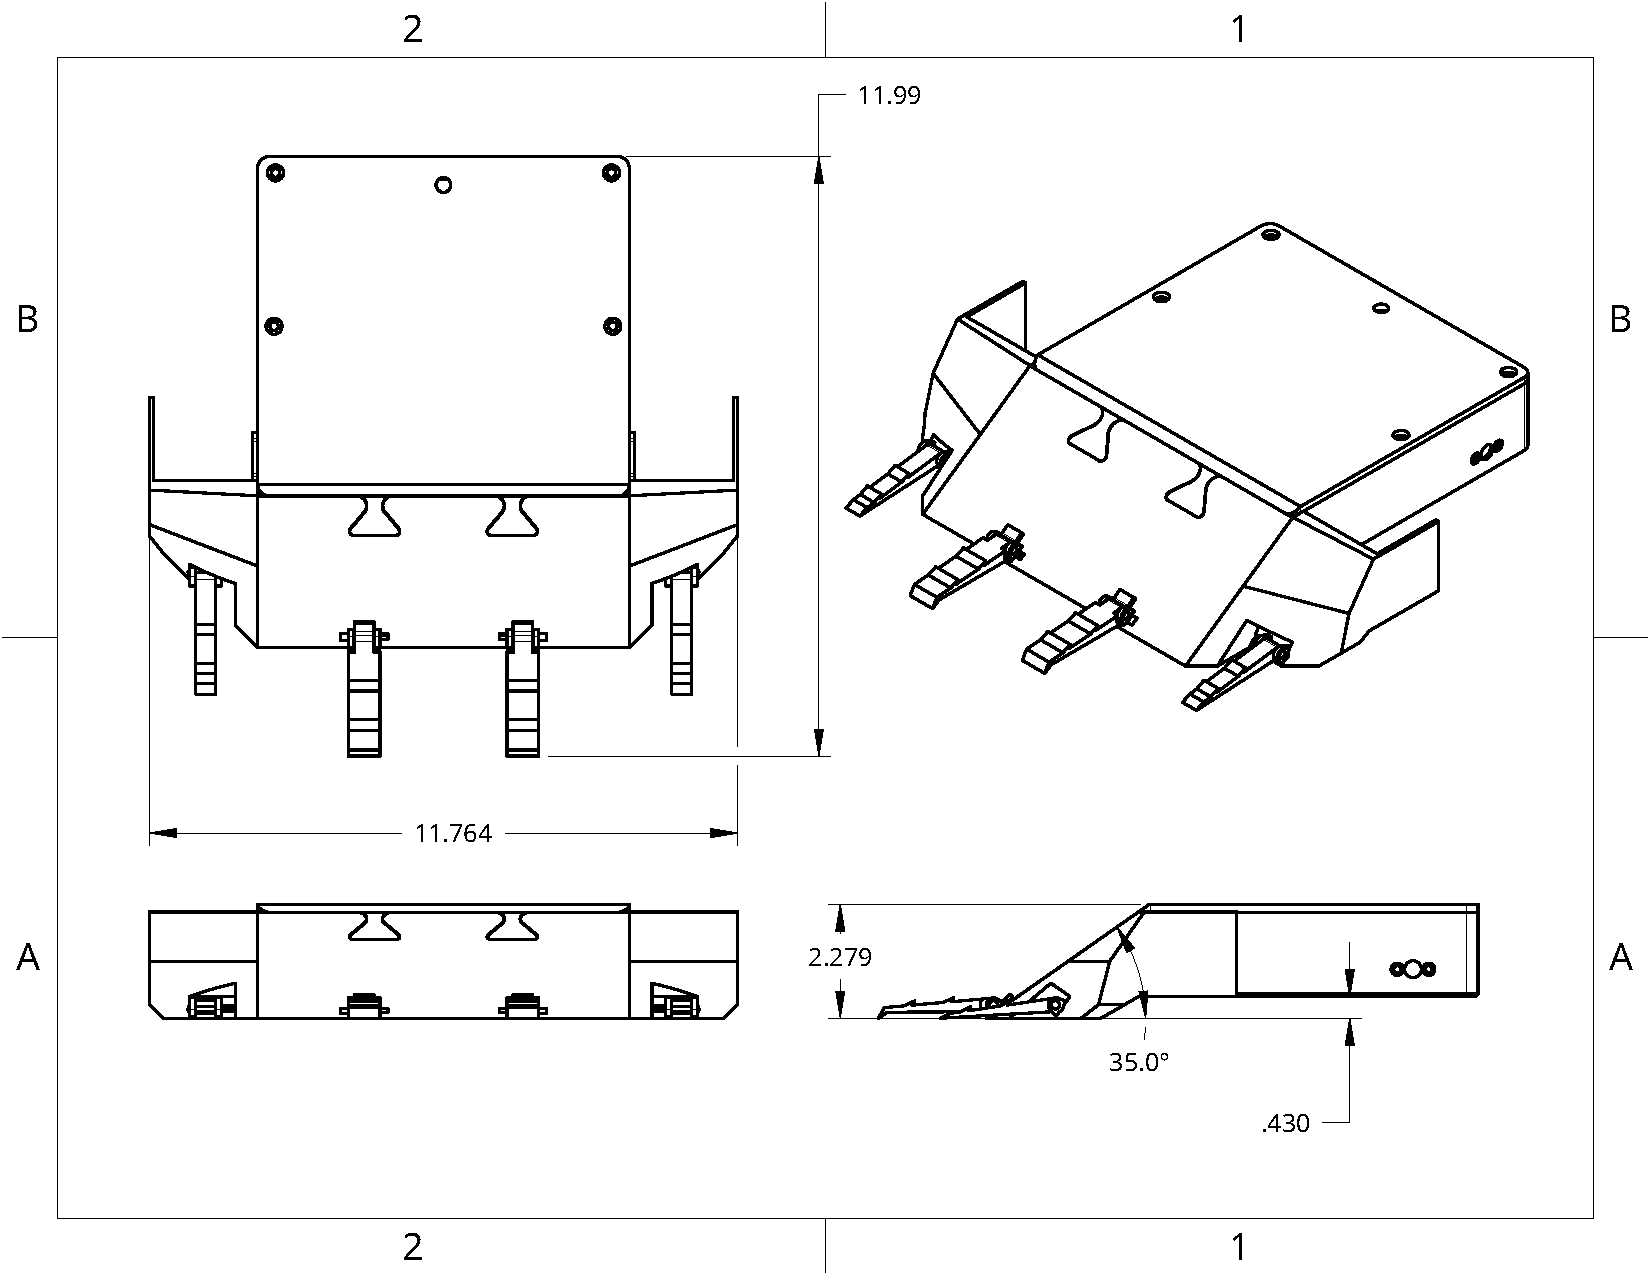
\includegraphics[width=0.8\textwidth]{fig_chassis_dimensions.pdf}
  \caption{Dimensioned drawing of the chassis, in inches. These are the nominal CAD dimensions. Sizes quoted in the text are measured on the built robot and differ from these by print tolerance; the forks and wedge are slightly undersize so they have clearance in their fittings.}
  \label{fig:dimensions}
\end{figure}

\subsection{Wedge and fork geometry}
\label{sec:wedge}

We set the wedge and fork angles from the ramp angle. \tbd{Explain the \mbox{\ang{33}}, \mbox{\ang{57}} and \mbox{\ang{147}} construction from the notebook sketch, what the vulnerability window is, and why the minimum fork angle is \mbox{\ang{33}}.} We left the edge slightly blunt so it would not snap. The forks are shaped to sit flush on the mesa while the tracks are still on the ramp, so the front edge is never raised as the robot arrives (Fig.~\ref{fig:wedge}).

\begin{figure}[htbp]
  \centering
  \placeholderfig{2.2in}{\textbf{\large Figure: drawing here}\\[4pt]Wedge and fork geometry: the \ang{33}, \ang{57} and \ang{147} construction, and the forks sitting flush on the mesa while the tracks are still on the ramp.}
  \caption{\tbd{Drawing of the wedge and fork geometry: the \mbox{\ang{33}}, \mbox{\ang{57}} and \mbox{\ang{147}} construction, and the forks sitting flush on the mesa while the tracks are still on the ramp.}}
  \label{fig:wedge}
\end{figure}

\subsection{Failure Analysis: Shaft couplers}
\label{sec:couplers}

Printed couplers join each motor's \qty{4}{mm} D-shaft to the stock sprocket (Fig.~\ref{fig:coupler}). Each is \qty{25.3}{mm} long and \qty{7.8}{mm} in diameter, round with one flat, and it works as a shaft collar and an adapter at once. The motor shaft fills a \qty{9.3}{mm} deep D-shaped bore at one end and is clamped by a set screw. The outside of the coupler, with its flat, extends the motor's small D-shaft into the larger D-shaped bore of the sprocket, which fits over the first \qty{8}{mm} at the other end, and a self-tapping screw driven into the \qty{1.6}{mm} pilot hole along the axis fastens the sprocket on.

The tracks have to be tight so they do not dip and scrape at the mesa edge. The first couplers, printed standing up, snapped under that tread tension, most of them during assembly rather than in operation. After the contest we treated the coupler as a cantilever and found the largest tread tension it can carry in each print orientation, to see whether orientation explains why those couplers broke and the reprints held.

3D-printed parts are much weaker across their layers than along them, because only the bond between layers resists stress normal to the layer planes. A coupler printed standing up, with its axis along the build direction, carries its bending stress straight across the layer bonds. One printed lying down carries it along the extruded lines (Fig.~\ref{fig:coupler}).

\begin{figure}[htbp]
  \centering
  \placeholderfig{2.2in}{\textbf{\large Figure: drawing here}\\[4pt]Coupler section view from CAD for both print orientations, showing layer direction, shaft bore, sprocket and the load at lever arm $\ell$.}
  \caption{\tbd{Side-by-side slicer views of the coupler printed upright and lying down, with the layer lines visible.}}
  \label{fig:coupler}
\end{figure}

Only one span of the coupler can break. Over its first \qty{8}{mm} it sits inside the rigid sprocket bore, and over its last \qty{9.3}{mm} it wraps the steel motor shaft, which carries the bending there. From 8 to \qty{16}{mm} the plastic carries the load alone.

The tread pulls on the sprocket with a total force $T$, perpendicular to the shaft. Along the free span the bending moment grows toward the motor, so it peaks at the bottom of the motor bore, a distance $\ell$ from the line of the tread. The peak bending stress there is
\begin{equation}
  \sigma = \frac{M c}{I} = \frac{T \ell c}{I}
  \label{eq:bending}
\end{equation}
and the largest pull it can carry before failing is
\begin{equation}
  T_\mathrm{max} = \frac{\sigma_\mathrm{allow}\,(I/c)}{\ell}
  \label{eq:tmax}
\end{equation}
The section at the bottom of the bore is the full D profile with the \qty{1.6}{mm} pilot hole. The coupler turns with the shaft, so the load passes through every direction once per revolution. The worst direction puts the peak stress at a corner of the flat, where $I/c = \qty{36.7}{mm^3}$. The tread runs somewhere on the sprocket's \qty{8}{mm} hub, so $\ell$ lies between 8 and \qty{16}{mm} \tbd{confirm where the tread runs on the hub}.

% no, this is still tread tension - to get the tread *over* and onto the undriven wheel requires significantly more displacement than it just sitting there, you have to force it on even with the slot
Assembly can also bend the coupler with no tread tension at all. A sideways push on the sprocket rim, parallel to the shaft, bends the free span with a lever arm equal to the \qty{25}{mm} sprocket radius, so Eq.~\eqref{eq:tmax} applies with $\ell = \qty{25}{mm}$.

% we didn't use ultimaker PLA and lab tests usually come up with much less optimistic values. Find and use better data.
The two orientations fail in different ways. Printed upright, PLA fractures across its layers without yielding first, so for the upright print $\sigma_\mathrm{allow}$ is its tensile strength at break. Printed flat, it yields first and fractures only after several percent more strain, so the lying print does not snap at its limit: it bends permanently, at its yield strength. Both values come from the Ultimaker PLA data sheet~\cite{ultimaker} \tbd{confirm our filament brand}. Transverse shear is at most \qty{15}{\percent} of the bending stress over this range of $\ell$, and the motor's stall torque of about \qty{0.2}{N.m} adds only about \qty{3}{MPa} of shear, so bending governs.

\begin{table}[htbp]
  \centering
  \caption{Force on the sprocket at which each print orientation fails (upright by fracture, lying by yielding), $T_\mathrm{max}$ from Eq.~\eqref{eq:tmax} with $I/c = \qty{36.7}{mm^3}$.}
  \label{tab:coupler}
  \begin{tabular}{@{}l c c@{}}
    \toprule
    & Upright: stress & Lying: stress \\
    & across the layers & along the layers \\
    \midrule
    $\sigma_\mathrm{allow}$~\cite{ultimaker} (\unit{MPa}) & 33.1, fracture & 52.5, yield (no fracture) \\
    \midrule
    Tread line at the inner edge of the hub, $\ell = \qty{8}{mm}$ & \qty{152}{N} (\qty{34}{\lbf}) & \qty{241}{N} (\qty{54}{\lbf}) \\
    Tread line at mid-hub, $\ell = \qty{12}{mm}$ & \qty{101}{N} (\qty{23}{\lbf}) & \qty{161}{N} (\qty{36}{\lbf}) \\
    Tread line at the outer face, $\ell = \qty{16}{mm}$ & \qty{76}{N} (\qty{17}{\lbf}) & \qty{120}{N} (\qty{27}{\lbf}) \\
    Sideways push on the sprocket rim, $\ell = \qty{25}{mm}$ & \qty{49}{N} (\qty{11}{\lbf}) & \qty{77}{N} (\qty{17}{\lbf}) \\
    \bottomrule
  \end{tabular}
\end{table}

Lying down, the coupler carries 1.6 times the load of the upright print before it fails, and it then bends instead of snapping. We reprinted the couplers lying down and they did not break again.

We never measured the forces during assembly, so Table~\ref{tab:coupler} compares the two orientations rather than predicting when either breaks. Ultimaker's specimens are printed at \qty{100}{\percent} infill with tuned settings, so our couplers were likely weaker than these values \tbd{confirm our print settings}. In operation the coupler is also bent back and forth once per revolution, so it could fail by fatigue below them.

\section{Electronics and power}
\label{sec:electronics}

\subsection{Architecture}
\label{sec:architecture}

Figure~\ref{fig:electronics} shows the wiring. A Particle Photon~2~\cite{photon2} runs the robot. It replaced the kit's ESP32 board, which failed during bench wiring for reasons we could not determine. The kit's motor shield drives its motors through a co-processor commanded over a serial link; we replaced it with a SparkFun TB6612FNG dual motor driver~\cite{sparkfun} we had on hand, controlled directly from the Photon's pins and with its motor supply wired straight to the battery. An MPU6050~\cite{mpu6050} gyro and accelerometer on the I$^2$C bus does all the sensing, read by firmware written mostly with Claude Code~\cite{claude}. Power comes from the supplied 2S pack of 18650 cells \tbd{confirm capacity: 2,500 or 3,000 mAh}. A judge starts the run with a single switch, which the Photon reads directly.

\begin{figure}[htbp]
  \centering
  \definecolor{packred}{HTML}{E8402F}\definecolor{fiveorange}{HTML}{E08A00}\definecolor{logicblue}{HTML}{1F6FB4}
  \begin{tikzpicture}[font=\small,
      box/.style={draw=black,line width=0.8pt,rounded corners=2pt,fill=black!4,align=center,minimum height=1.3cm,text width=2.5cm},
      pack/.style={line width=1.6pt,draw=packred,-{Latex[length=2.2mm]}},
      five/.style={line width=1.6pt,draw=fiveorange,-{Latex[length=2.2mm]}},
      logic/.style={line width=1.2pt,draw=logicblue,-{Latex[length=2.2mm]}},
      sig/.style={line width=1.0pt,draw=black,-{Latex[length=2.2mm]}}]
    \node[box,fill=black!2,text width=2.3cm] (pack) at (0,0) {\textbf{2S pack}\\two 18650 cells};
    \node[box] (reg) at (3.4,1.6) {\textbf{7805}\\regulator};
    \node[box] (sw) at (3.4,-0.6) {\textbf{Start switch}};
    \node[box,minimum height=4.2cm,text width=2.4cm,fill=black!2] (mcu) at (8.4,0.2) {\textbf{Photon 2}\\controller\\(\qty{3.3}{V} logic)};
    \node[box] (imu) at (13.2,1.6) {\textbf{MPU6050}\\gyro and\\accelerometer};
    \node[box,text width=2.9cm] (drv) at (13.2,-1.6) {\textbf{TB6612FNG}\\dual motor driver};
    \node[box,text width=1.4cm,minimum height=1cm] (ml) at (12.3,-3.8) {\textbf{Left}\\motor};
    \node[box,text width=1.4cm,minimum height=1cm] (mr) at (14.1,-3.8) {\textbf{Right}\\motor};
    \draw[pack] (pack.north) |- node[pos=0.75,above,text=packred] {pack} (reg.west);
    \draw[five] (reg.east) -- node[above,text=fiveorange] {\qty{5}{V} (VUSB)} (reg.east -| mcu.west);
    \draw[sig] (sw.east) -- node[above] {digital in} (sw.east -| mcu.west);
    \draw[logic,{Latex[length=2.2mm]}-{Latex[length=2.2mm]}] (imu.west -| mcu.east) -- node[above,text=logicblue] {I$^2$C} (imu.west);
    \draw[logic] ([yshift=0.3cm]drv.west -| mcu.east) -- node[above,text=logicblue] {control} ([yshift=0.3cm]drv.west);
    \draw[pack] (pack.south) |- node[pos=0.75,below,text=packred] {VM: pack voltage (motor supply)} (11.0,-2.7) |- ([yshift=-0.35cm]drv.west);
    \draw[sig] (ml.north |- drv.south) -- (ml.north);
    \draw[sig] (mr.north |- drv.south) -- (mr.north);
  \end{tikzpicture}
  \caption{Electronics block diagram. The 2S pack feeds the motor driver directly and the Photon~2 through the 7805 regulator. The Photon reads the MPU6050 over I$^2$C and drives the TB6612FNG.}
  \label{fig:electronics}
\end{figure}

The TB6612FNG switches the motors with MOSFETs and loses about \qty{0.5}{V} at \qty{1}{A}, against about \qty{2}{V} for the bipolar L298 used on many hobby driver boards, so more of the pack voltage reaches the motors~\cite{tb6612,l298}.

The Photon takes \qty{5}{V} on its VUSB pin and makes its own \qty{3.3}{V} for logic, so every sensor and signal line runs at \qty{3.3}{V}. A 7805 linear regulator makes the \qty{5}{V} from the pack. It needs about \qty{2}{V} of headroom, so it holds \qty{5}{V} only while the pack stays above about \qty{7}{V}; a 2S pack runs from \qty{8.4}{V} full to about \qty{6.4}{V} empty~\cite{cell}. We bench-tested the regulator with the capacitors we had, two \qty{100}{nF} in parallel on the input and one \qty{100}{nF} on the output, below the \qty{0.33}{\micro F} input capacitor the datasheet calls for~\cite{reg7805}, and measured \qty{5.05}{V} out.

\subsection{Resets from a loose cell}
\label{sec:resets}

During bench testing the Photon sometimes restarted when the robot was jolted. Stalling both motors never caused a restart, but snapping the robot back and forth by hand with the motors idle did, which ruled out a supply dip from motor current. The cells sit in a plastic holder with spring contacts, and the jolt let a cell compress its spring far enough to lose contact for an instant. Fastening the holder so it could not snap against its stop ended the restarts \tbd{confirm}.

\section{Sensing the crest}
\label{sec:sensing}

\subsection{Why an accelerometer alone is not enough}
\label{sec:accel-only}

% add vector angle equation and use z hat notation for z vector
The robot has to know when it has crossed from the \ang{33.4} ramp onto the flat mesa, and it has to know this while speeding up and slowing down. An accelerometer reads acceleration along three basis vectors. At standstill, resultant acceleration vector retrieved is the gravity vector, from which it's trivial to calculate the robot's tilt: simply take the angle between the z vector and gravity vector.
However, when the robot accelerates along the ramp, the resultant vector ceases to be the gravity vector.

Along the ramp it reads $g \sin\ang{33.4} + a$ and across it $g \cos\ang{33.4}$, so the pitch it implies is
\begin{equation}
  \theta_\mathrm{apparent} = \arctan\!\left(\frac{g \sin\ang{33.4} + a}{g \cos\ang{33.4}}\right)
  \label{eq:apparent}
\end{equation}
Table~\ref{tab:apparent} shows the size of the error. Decelerating at \qty{3}{m/s^2} makes the ramp look like \ang{16}, below the \ang{18} threshold at which our robot decides it has crested.

\begin{table}[htbp]
  \centering
  \caption{Pitch an accelerometer alone reports on the \ang{33.4} ramp.}
  \label{tab:apparent}
  \begin{tabular}{@{}l cccccc@{}}
    \toprule
    $a$ along the ramp (\unit{m/s^2}) & $-3$ & $-2$ & $-1$ & 0 & $+1$ & $+2$ \\
    \midrule
    Apparent pitch (\unit{\degree}) & 16.3 & 22.5 & 28.2 & 33.4 & 38.0 & 42.1 \\
    \bottomrule
  \end{tabular}
\end{table}

% hold on wait a minute
% lowk why didn't we just solve this numerically for theta given that the acceleration in the x direction is known to be always 33deg up
% uhhhhhhhhh
A gyroscope measures rotation rate directly and is not fooled by linear acceleration, but turning its rate into an angle means integrating, and integration accumulates error. Ours read up to \qty{4.7}{\degree/s} with the robot at rest; over a \qty{5}{s} climb that offset alone would add \ang{23} of error.

\subsection{Complementary filter}
\label{sec:filter}

We combine the two sensors with a complementary filter that tracks the direction of gravity as a unit vector $\bm{u}$ in the sensor's frame, in the form of Mahony's explicit complementary filter~\cite{mahony}. Every \qty{20}{ms} the gyro rate $\bm{\omega}$ rotates the estimate, and the result is renormalized:
\begin{equation}
  \bm{u} \leftarrow \operatorname{normalize}\!\big(\bm{u} - (\bm{\omega} \times \bm{u})\,\Delta t\big)
  \label{eq:gyro-step}
\end{equation}
When the accelerometer reading $\hat{\bm{a}}$ can be trusted, the estimate is then pulled toward it with a time constant $T_c = \qty{1.5}{s}$:
\begin{equation}
  \bm{u} \leftarrow \operatorname{normalize}\!\left(\bm{u} + \frac{\Delta t}{T_c}\left(\frac{\hat{\bm{a}}}{|\hat{\bm{a}}|} - \bm{u}\right)\right)
  \label{eq:accel-step}
\end{equation}
The accelerometer is trusted only while its reading is within \qty{8}{\percent} of \qty{1}{g}, the rotation rate is below \qty{30}{\degree/s}, and the motor commands have been steady for \qty{0.6}{s}. In every other moment the estimate follows the gyro alone. The gyro offset is averaged over 50 readings with the robot at rest and subtracted from every reading after that. A two-step calibration (robot level, then nose up) gives the robot its own up and forward directions, from which it computes pitch.

\subsection{Requirement and test}
\label{sec:pitch-test}

The autopilot decides it has crested when the pitch stays below \ang{18} for \qty{40}{ms}, and on the mesa it counts anything within \ang{\pm 6} as level. The estimate therefore must not read more than \ang{15} low while climbing the \ang{33.4} ramp, and must be within \ang{\pm 6} at rest. \tbd{Confirm these were the thresholds used in the contest.}

To test this we used the hill itself as ground truth: anywhere on the ramp the true pitch is \ang{33.4}, and on the mesa it is \ang{0}. We logged both the accelerometer-only and the fused pitch through three full autonomous runs (Fig.~\ref{fig:pitch}, Table~\ref{tab:pitch}). Climbing, the accelerometer alone was off by up to \ang{122}, while the fused estimate never read more than \ang{4.5} from the true angle, well inside the \ang{15} the crest test allows. At rest, both were within \ang{4} on the mesa, inside the \ang{\pm 6} level band.

\begin{figure}[htbp]
  \centering
  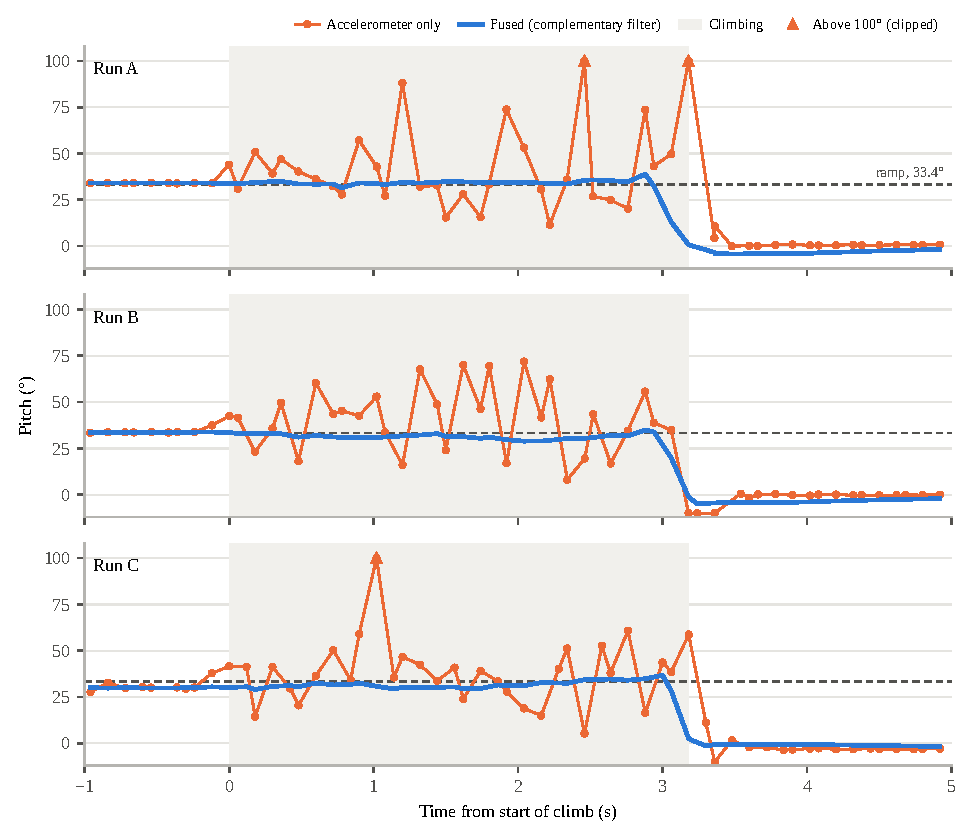
\includegraphics[width=0.92\textwidth]{fig11_pitch.pdf}
  \caption{Pitch during three autonomous climbs. Under full power the accelerometer alone reads anywhere from \ang{5} to over \ang{150}, while the fused estimate stays within \ang{4.5} of the true \ang{33.4} until the crest.}
  \label{fig:pitch}
\end{figure}

\begin{table}[htbp]
  \centering
  \caption{Pitch error against the known hill angle (\ang{33.4} on the ramp, \ang{0} on the mesa). Climbing uses all three runs; the rest rows use Runs A and B, since Run C started off the ramp face.}
  \label{tab:pitch}
  \begin{tabular}{@{}l cc cc@{}}
    \toprule
    & \multicolumn{2}{c}{Accelerometer only} & \multicolumn{2}{c}{Fused} \\
    \cmidrule(lr){2-3}\cmidrule(l){4-5}
    Condition & Max.\ error & RMS & Max.\ error & RMS \\
    \midrule
    At rest on the ramp       & \ang{0.8}   & \ang{0.5}  & \ang{0.6} & \ang{0.5} \\
    Climbing under full power & \ang{121.7} & \ang{24.0} & \ang{4.5} & \ang{2.1} \\
    At rest on the mesa       & \ang{0.8}   & \ang{0.5}  & \ang{3.9} & \ang{1.6} \\
    \bottomrule
  \end{tabular}
\end{table}

\section{Autonomous control}
\label{sec:control}

\subsection{The run: climb, decelerate, hold}
\label{sec:run}

An autonomous run has three stages (Fig.~\ref{fig:states}). In Climb, both motors run at full power. The robot has no way to measure distance, so Climb ends as soon as either of two conditions is met: \qty{3.15}{s} have passed since the start, or the pitch has stayed below \ang{18} for \qty{40}{ms}. The robot ignores the pitch condition for the first \qty{0.3}{s} of the run. In Decelerate, the drive power ramps linearly from full to zero over a set time, and momentum carries the robot from the ridge onto the mesa. It then enters Hold.

In Hold, the robot sets its motor power to zero while it is level, and the driver code applies zero power as short brake. Short brake connects each motor's two terminals together. A motor turned by an outside force then acts as a generator driving current through its own windings, and that current makes a torque opposing the motion, $\tau_\mathrm{brake} = k_\mathrm{t}^2 \omega / R_\mathrm{w}$ for a motor turned at speed $\omega$.

Hold also corrects the robot's position from its pitch. If the nose rises more than \ang{6}, because the robot stopped short of the top or is being shoved back down our ramp, it drives forward at full power, 255 of 255. If the nose drops more than \ang{6}, because the robot is about to go over the far side, it backs up at 110 of 255. It keeps correcting until the pitch is back within \ang{3}, so that it does not switch rapidly between correcting and braking at the edge of the \ang{6} band.

\begin{figure}[htbp]
  \centering
  \begin{tikzpicture}[
      font=\small,
      >={Stealth[length=2.4mm]},
      every edge/.style={draw,->,thick},
      state/.style={draw,thick,rounded corners=3pt,align=center,
                    text width=3.3cm,minimum height=1.35cm,inner sep=3pt},
      wait/.style={state,fill=black!6},
      run/.style={state,fill=blue!12},
      lbl/.style={align=center,font=\footnotesize,inner sep=2pt},
    ]
    \node[wait] (armed) at (0,0)       {\textbf{Armed}\\motors short-braked, holding the robot on the ramp};
    \node[run]  (climb) at (5.6,0)     {\textbf{Climb}\\both motors at full power (255)};
    \node[run]  (dec)   at (5.6,-3.5)  {\textbf{Decelerate}\\power ramps linearly to zero over \qty{150}{ms}};
    \node[run]  (hold)  at (5.6,-6.9)  {\textbf{Hold}\\motors short-braked};
    \node[run]  (back)  at (0,-6.9)    {\textbf{Back up}\\power 110};
    \node[run]  (fwd)   at (11.2,-6.9) {\textbf{Drive forward}\\power 255};

    \draw[->,thick] (armed) -- node[lbl,above] {start switch\\on} (climb);

    \draw[->,thick] (climb.north east) ++(-0.5,0)
      .. controls +(0.6,1.3) and +(-0.6,1.3) .. ([xshift=0.5cm]climb.north west)
      node[lbl,pos=0.5,above] {neither condition met};

    \draw[->,thick] (climb) -- node[lbl,right,align=left]
      {\qty{3.15}{s} after the start\\\textbf{or} pitch below \ang{18} for \qty{40}{ms}\\(pitch tested after the first \qty{0.3}{s})} (dec);

    \draw[->,thick] (dec) -- node[lbl,right,pos=0.35] {power at zero} (hold);

    \draw[->,thick] (hold.15) to[bend left=28] node[lbl,above] {nose up more\\than \ang{6}} (fwd.165);
    \draw[->,thick] (fwd.195) to[bend left=28] node[lbl,below] {back within\\\ang{3}} (hold.345);

    \draw[->,thick] (hold.165) to[bend right=28] node[lbl,above] {nose down more\\than \ang{6}} (back.15);
    \draw[->,thick] (back.345) to[bend right=28] node[lbl,below] {back within\\\ang{3}} (hold.195);

    \begin{scope}[shift={(9.6,0.55)},font=\footnotesize]
      \node[draw,fill=black!6,minimum size=2.6mm,inner sep=0pt] (k1) at (0,0) {};
      \node[anchor=west] at (0.2,0) {waiting for the start};
      \node[draw,fill=blue!12,minimum size=2.6mm,inner sep=0pt] (k2) at (0,-0.5) {};
      \node[anchor=west] at (0.2,-0.5) {autonomous run};
    \end{scope}
  \end{tikzpicture}
  \caption{The autonomous run. Climb ends on time or on pitch, whichever comes first. In Hold the robot reacts to pitch alone.}
  \label{fig:states}
\end{figure}

\subsection{Tuning}
\label{sec:tuning}

We empirically found that a climb takes about \qty{3.3}{s}, so we set \qty{3150}{ms} of full-power climb and a \qty{150}{ms} deceleration ramp. We also built a trim tool for straight-line driving that works as a binary search: each press shifts power \qty{16}{\percent} toward the lagging side, and the step halves every time the drift reverses. The side wall keeps the robot on a straight line either way, but a robot that pulls toward the wall spends power pushing itself into it, which only slows the climb. Trimming the motors to drive straight puts that power back into climbing.

At first, Hold corrected at full power, 255, in both directions. The robot then oscillated on the mesa: it threw itself forward, overshot, threw itself back, overshot, and so on. We lowered the back-up power to 110 to stop this, and kept forward correction at full power.

From our average climb speed of \qty{0.46}{m/s}, stopping takes $v^2/(2a)$: \qty{11}{cm} at \qty{1}{m/s^2} and \qty{4}{cm} at \qty{3}{m/s^2}, both inside the \qty{30}{cm} mesa. We never ran the robot without the Decelerate stage, so we cannot say whether overshooting the mesa was a real risk.

\section{Testing summary}
\label{sec:testing}

Table~\ref{tab:tests} lists every test, what it varied and measured, and the decision it drove. Tests marked ``new'' were run after the contest for this report.

\begin{table}[htbp]
  \centering
  \caption{All tests, with the cause (what we varied) to the left of the effect.}
  \label{tab:tests}
  {\small
  \begin{tabularx}{\textwidth}{@{}>{\raggedright\arraybackslash}p{0.17\textwidth} L L L L@{}}
    \toprule
    Test & What we varied & What we measured & Result & Decision it drove \\
    \midrule
    Stall current & none & Current at stall & \qty{1.4}{A} per motor & Acceptable for brief stalls \\
    Regulator bench test & none & Output voltage & \qty{5.05}{V} & Safe to power the Photon through VUSB \\
    Resets under impulse & Motors driven vs.\ idle, hand rotation & Whether the Photon restarted & Restarted with motors idle & Fastened the battery box and cells \\
    Timed climbs & none & Climb time by stopwatch & about \qty{3.3}{s} & Set the Climb backstop \tbd{to \mbox{\qty{3000}{ms}}} \\
    Straight-line trim & Power split between motors & Drift direction & \tbd{\ } & \tbd{\ } \\
    Friction (new) & Surface, normal force & Friction force at slip & \tbd{\ } & \tbd{\ } \\
    Pitch accuracy (new) & Known angles and paths & Pitch error & \tbd{\ } & \tbd{\ } \\
    Hold strength (new) & Short brake vs.\ open terminals vs.\ hold active & Force to push off the mesa & \tbd{\ } & \tbd{\ } \\
    \bottomrule
  \end{tabularx}
  }
\end{table}

% drift direction correction values should be stored in code
% you have the data to fill in pitch accuracy, in terms of decision it drove, nothing - determination that simple filter good enough
% retain the hold strength and friction rows for now, but likely we won't have time to get around to these

\section{Contest results}
\label{sec:results}

We won the contest with a 5--1 record (Table~\ref{tab:rounds}). The competition score is $50P/M + 50$, where $P$ is our points in the Swiss tournament (1 per win) and $M$ is the most points any team received. As the winners we had the most points, so $P = M = 5$ and the score is 100.

\begin{table}[htbp]
  \centering
  \caption{Contest rounds.}
  \label{tab:rounds}
  {\small
  \begin{tabularx}{\textwidth}{@{}c l L L@{}}
    \toprule
    Round & Opponent & Outcome & Why \\
    \midrule
    1 & Team 11 & Won. Our car arrived at the top before team 11. When the cars met, our car pushed back against the force they exerted and got team 11's car on top of ours. Our farthest point was closer, so we won. & The gearmotors got us to the top first, and the forks and wedge plate let team 11's car go over us instead of pushing us off. \\
    2 & Team 08 & Won. Team 08 reached the top first, but went over our car and fell to the end of the ramp, unable to come back. & The forks and wedge plate let the car go over us instead of pushing us off. \\
    3 & Team 09 & Won. We reached the top first and stayed closer to it. The match was close, because both cars ended near the center. & The gearmotors got us to the top first, which gave us the upper hand. \\
    4 & Team 14 & Won. We got to the top first, and because team 14's car was easy for our ramp to get under, we kept our spot under them while they kept driving forward. & The gearmotors got us to the top first, and the low wedge plate slid under team 14's car, so we held our spot while they kept driving forward. \\
    5 & Team 10 & Won. We reached the top later than team 10, but their strategy was to keep going and never stop. Our forks got their car onto ours, and team 10 drove past us and off the ramp. & The forks and wedge plate let the car go over us instead of pushing us off. \\
    6 & Team 05 & Lost. We reached the mesa first and got under the opponent, but stopped short, and its farthest point was closer to the center. & Advance onto the mesa timed, not measured (Section~\ref{sec:lessons}) \\
    \bottomrule
  \end{tabularx}
  }
\end{table}

Our one loss, in the final round, came from the robot's timed advance onto the mesa (Section~\ref{sec:lessons}). We reached the mesa first and got under the opponent, as designed, but the robot stopped short of where it usually did. The opponent's footprint was much smaller than ours, so its farthest point was closer to the mesa center, and we lost on that rule.

\begin{figure}[htbp]
  \centering
  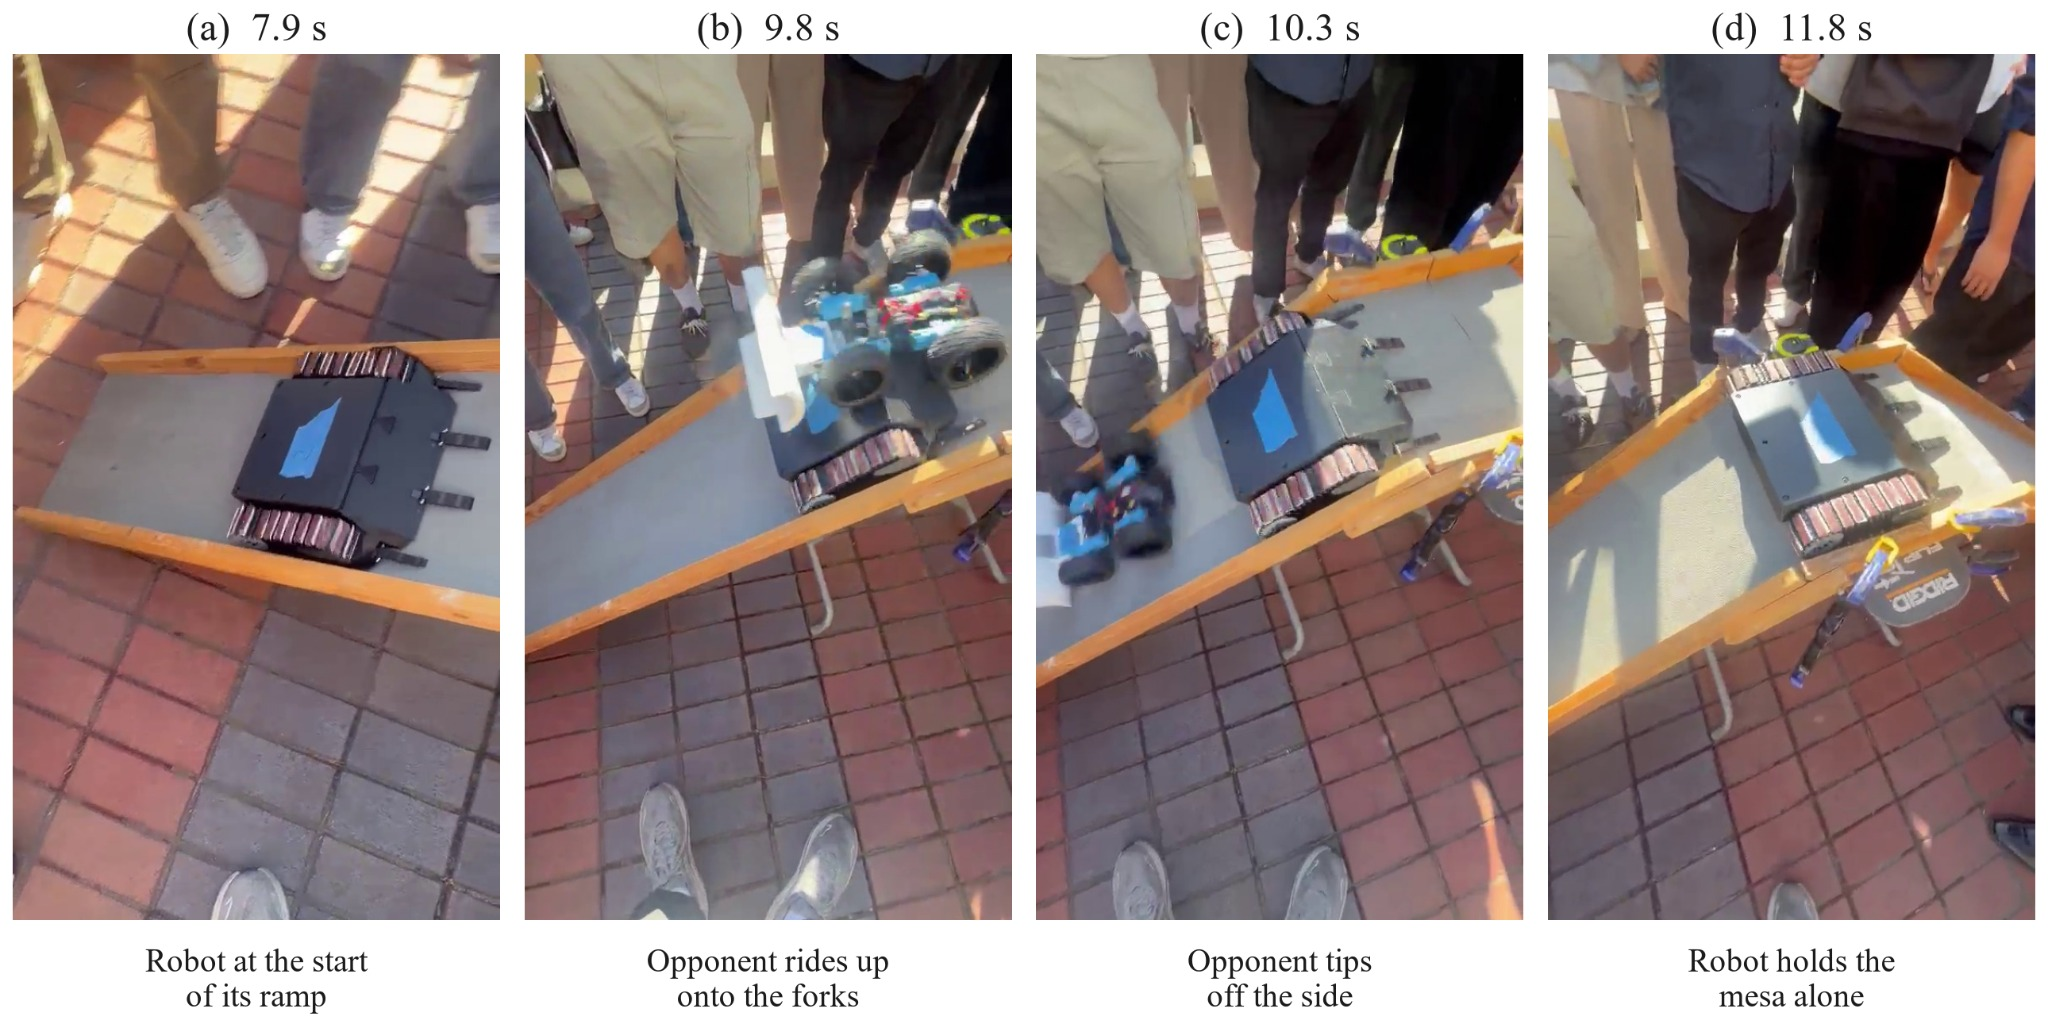
\includegraphics[width=0.9\textwidth]{fig13_contest.jpg}
  \caption{Frames from Round \tbd{N}, left to right. An opponent drives up onto our forks and tips off the side, and our robot holds the mesa alone.}
  \label{fig:contest}
\end{figure}

\section{Lessons learned}
\label{sec:lessons}

\paragraph{Triage, and build the minimum viable robot first}
% the construction of these sentences gets so convoluted that it becomes impossible to tell between things that were actually done or considered but dropped
This is the lesson that mattered most. We dropped ideas that were too complex for the time we had (the servo wall brace and the side lifter), and chose not to fix some things we knew were imperfect: side guards that wrapped fully around the treads (we had CAD for them, but they were too ambitious to make work in time), a ground-up sprocket redesign for a controlled diameter, proper electronics mounts in place of hot glue, metal couplers that would not deflect, a soldered protoboard, and modular wedges. That kept enough time to test the robot and its software, and without that testing the autonomous run would not have worked.

\paragraph{Isolate faults one connection at a time}
Our two longest debugging sessions were a breadboard jumper whose trimmed leg never seated and a cold solder joint on the IMU's power header. Both passed every check we made until we measured the voltage at each connection in turn, from the supply to the part.

\paragraph{Check stiffness as well as strength}
The side guards we cut down to fit never broke, but they flexed into the treads and dragged on them in every run. The motors had the margin to push through it (Section~\ref{sec:drivetrain-result}), but a part that bends too far can stop doing its job long before it breaks.

\paragraph{Take print anisotropy seriously}
We printed both coupler orientations and chose the upright one because the fit felt marginally nicer, and we guessed by feel that it would be strong enough, even in the anisotropically weaker configuration. For load-bearing functional parts, a guess isn't good enough: upright-printed couplers almost all broke.

% I just remembered - a very plausible hypothesis for why our little pushing past the mesa edge could've become less is because the *treads themselves lose tension over successive runs, and we could actually feel this happening*
% Oddly not at the slots, *at the couplers* (which were literally bent by like maybe 2-5 degrees, just super guessing visually from memory)
\paragraph{Autonomy without positioning suffers}
The advance past the crest was set by time, so anything that changed the robot's speed, such as vibration, track slip, or an opponent, changed where it stopped. Wheel or motor encoders would not fix this, because they cannot tell when the tracks slip. An absolute position reference would: a time-of-flight sensor ranging to a beacon, or a camera such as an ESP32-CAM locating AprilTags on the side walls. We had hoped to build one but ran out of time.

% this was a 1-off 3-minute debug for a scenario (high lateral g) that never would even happen in comp, why is this in the all-time lessons list
\paragraph{Fully constrain electronics}
The battery cells sat in a plastic holder with spring contacts. A sharp jolt let a cell compress its spring past the contact's interference and lose contact for an instant, which restarted the controller. Fastening the holder so it could not take shock loads stopped the restarts.

\paragraph{Spend analysis where the eye cannot see}
Many questions answered themselves by inspection: whether the tracks slipped, whether the robot tipped, whether it stopped on the mesa. We judged or tuned those by eye, which was good enough, and saved more rigorous analysis for tradeoffs that cannot be eyeballed, such as the gear ratio (Section~\ref{sec:gear-ratio}) and battery voltage sag (Section~\ref{sec:current-bound}) \tbd{finish this list}.

\section{Conclusion}
\label{sec:conclusion}

Our objective was to reach the mesa first and keep the opponent from displacing us for the rest of the \qty{30}{s}. Three decisions mattered most: a low wedge with forks that neutralizes an opponents' drive force, larger motors at an optimal gear ratio, and a pitch estimate that fuses the gyro and accelerometer so the robot can hold its place on the mesa. The robot won the contest with a 5--1 record, and its one loss came from pacing the climb by time, which left the robot short on the mesa. If we built it again, we would measure position instead of timing the climb.

% ASME numbered references, listed in order of first citation.
% Numbers are assigned automatically from this order; cite by key with \cite{}.

\clearpage
\renewcommand{\refname}{References}
\begin{thebibliography}{99}
\addcontentsline{toc}{section}{References}
\setlength{\itemsep}{2pt}
\small

\bibitem{ronney}
Ronney, P.~D., 2026, ``AME 101 Lecture Notes,'' University of Southern California, Los Angeles, CA.

\bibitem{tb6612}
Toshiba Corporation, 2007, ``TB6612FNG Driver IC for Dual DC Motor,'' Datasheet.
\url{https://cdn.sparkfun.com/assets/0/1/b/b/3/TB6612FNG.pdf}

\bibitem{pololu37d}
Pololu Corporation, n.d., ``37D Metal Gearmotors,'' accessed Oct.~26, 2026.
\url{https://www.pololu.com/category/116/37d-metal-gearmotors}

\bibitem{pololu25d}
Pololu Corporation, n.d., ``25D Metal Gearmotors,'' accessed Oct.~26, 2026.
\url{https://www.pololu.com/category/115/25d-metal-gearmotors}

\bibitem{meccanixity}
MECCANIXITY, 2026, ``DC 6V Gear Motor High Torque with Bracket, 25~mm Dia.,'' 12 to 1360~rpm versions, Amazon.com, accessed Oct.~25, 2026.
\url{https://www.amazon.com/s?k=MECCANIXITY+DC+6V+Gear+Motor+High+Torque+with+Bracket+25mm}

\bibitem{azadi}
Azadi, M., and Dadashi, A., 2022, ``Experimental Fatigue Dataset for Additive-Manufactured 3D-Printed Polylactic Acid Biomaterials Under Fully-Reversed Rotating-Bending Loadings,'' Data in Brief, 41, p.~107846.
\url{https://doi.org/10.1016/j.dib.2022.107846}

\bibitem{ezeh}
Ezeh, O.~H., and Susmel, L., 2018, ``On the Fatigue Strength of 3D-Printed Polylactide (PLA),'' Procedia Struct.\ Integrity, 9, pp.~29--36.
\url{https://doi.org/10.1016/j.prostr.2018.06.007}

\bibitem{photon2}
Particle Industries, 2024, ``Photon 2 Datasheet,'' Rev.~16.
\url{https://docs.particle.io/reference/datasheets/wi-fi/photon-2-datasheet/}

\bibitem{sparkfun}
SparkFun Electronics, n.d., ``TB6612FNG Hookup Guide.''
\url{https://learn.sparkfun.com/tutorials/tb6612fng-hookup-guide}

\bibitem{mpu6050}
InvenSense, 2013, ``MPU-6000 and MPU-6050 Product Specification,'' Document PS-MPU-6000A-00, Rev.~3.4.
\url{https://product.tdk.com/system/files/dam/doc/product/sensor/mortion-inertial/imu/data_sheet/mpu-6000-datasheet1.pdf}

\bibitem{claude}
Anthropic, 2026, ``Claude and Claude Code,'' AI assistants, used to write most of the robot firmware and the Bluetooth dashboard and to help with analysis and drafting this report.
\url{https://claude.com/product/claude-code}

\bibitem{l298}
STMicroelectronics, 2023, ``L298 Dual Full-Bridge Driver,'' Datasheet DS0218, Rev.~5.
\url{https://www.st.com/resource/en/datasheet/l298.pdf}

\bibitem{cell}
\tbd{18650 cell data sheet.}

\bibitem{reg7805}
\tbd{7805 regulator data sheet, for the manufacturer of our part.}

\end{thebibliography}

\clearpage
\appendix
\titleformat{\section}{\normalfont\large\bfseries}{Appendix \thesection:}{0.5em}{#1}

\section{Firmware}
\label{app:firmware}

The robot runs the Particle Photon~2 firmware in \texttt{photon/ble\_robot/src}. \tbd{These listings are the files as they stand now. Estimator.h and Autopilot.h were last changed Oct.~12--13, before the contest; ble\_robot.cpp and Capture.h were changed Oct.~23, after it, to add a high-rate data capture. Confirm this is the version to list.}

\subsection*{ble\_robot.cpp}
\lstinputlisting{code/ble_robot.cpp}

\subsection*{Estimator.h}
\lstinputlisting{code/Estimator.h}

\subsection*{Autopilot.h}
\lstinputlisting{code/Autopilot.h}

\subsection*{Capture.h}
\lstinputlisting{code/Capture.h}

\clearpage
\section{Raw test data}
\label{app:data}

\tbd{Run-log summaries and full test tables.}


\end{document}
